% Options for packages loaded elsewhere
\PassOptionsToPackage{unicode}{hyperref}
\PassOptionsToPackage{hyphens}{url}
%
\documentclass[
]{book}
\usepackage{lmodern}
\usepackage{amssymb,amsmath}
\usepackage{ifxetex,ifluatex}
\ifnum 0\ifxetex 1\fi\ifluatex 1\fi=0 % if pdftex
  \usepackage[T1]{fontenc}
  \usepackage[utf8]{inputenc}
  \usepackage{textcomp} % provide euro and other symbols
\else % if luatex or xetex
  \usepackage{unicode-math}
  \defaultfontfeatures{Scale=MatchLowercase}
  \defaultfontfeatures[\rmfamily]{Ligatures=TeX,Scale=1}
  \setmainfont[]{Arial}
  \setmonofont[]{Courier New}
\fi
% Use upquote if available, for straight quotes in verbatim environments
\IfFileExists{upquote.sty}{\usepackage{upquote}}{}
\IfFileExists{microtype.sty}{% use microtype if available
  \usepackage[]{microtype}
  \UseMicrotypeSet[protrusion]{basicmath} % disable protrusion for tt fonts
}{}
\makeatletter
\@ifundefined{KOMAClassName}{% if non-KOMA class
  \IfFileExists{parskip.sty}{%
    \usepackage{parskip}
  }{% else
    \setlength{\parindent}{0pt}
    \setlength{\parskip}{6pt plus 2pt minus 1pt}}
}{% if KOMA class
  \KOMAoptions{parskip=half}}
\makeatother
\usepackage{xcolor}
\IfFileExists{xurl.sty}{\usepackage{xurl}}{} % add URL line breaks if available
\IfFileExists{bookmark.sty}{\usepackage{bookmark}}{\usepackage{hyperref}}
\hypersetup{
  pdftitle={STAT 107 Outline of Class Notes},
  pdfauthor={Rebecca Kurtz-Garcia},
  hidelinks,
  pdfcreator={LaTeX via pandoc}}
\urlstyle{same} % disable monospaced font for URLs
\usepackage{color}
\usepackage{fancyvrb}
\newcommand{\VerbBar}{|}
\newcommand{\VERB}{\Verb[commandchars=\\\{\}]}
\DefineVerbatimEnvironment{Highlighting}{Verbatim}{commandchars=\\\{\}}
% Add ',fontsize=\small' for more characters per line
\usepackage{framed}
\definecolor{shadecolor}{RGB}{248,248,248}
\newenvironment{Shaded}{\begin{snugshade}}{\end{snugshade}}
\newcommand{\AlertTok}[1]{\textcolor[rgb]{0.94,0.16,0.16}{#1}}
\newcommand{\AnnotationTok}[1]{\textcolor[rgb]{0.56,0.35,0.01}{\textbf{\textit{#1}}}}
\newcommand{\AttributeTok}[1]{\textcolor[rgb]{0.77,0.63,0.00}{#1}}
\newcommand{\BaseNTok}[1]{\textcolor[rgb]{0.00,0.00,0.81}{#1}}
\newcommand{\BuiltInTok}[1]{#1}
\newcommand{\CharTok}[1]{\textcolor[rgb]{0.31,0.60,0.02}{#1}}
\newcommand{\CommentTok}[1]{\textcolor[rgb]{0.56,0.35,0.01}{\textit{#1}}}
\newcommand{\CommentVarTok}[1]{\textcolor[rgb]{0.56,0.35,0.01}{\textbf{\textit{#1}}}}
\newcommand{\ConstantTok}[1]{\textcolor[rgb]{0.00,0.00,0.00}{#1}}
\newcommand{\ControlFlowTok}[1]{\textcolor[rgb]{0.13,0.29,0.53}{\textbf{#1}}}
\newcommand{\DataTypeTok}[1]{\textcolor[rgb]{0.13,0.29,0.53}{#1}}
\newcommand{\DecValTok}[1]{\textcolor[rgb]{0.00,0.00,0.81}{#1}}
\newcommand{\DocumentationTok}[1]{\textcolor[rgb]{0.56,0.35,0.01}{\textbf{\textit{#1}}}}
\newcommand{\ErrorTok}[1]{\textcolor[rgb]{0.64,0.00,0.00}{\textbf{#1}}}
\newcommand{\ExtensionTok}[1]{#1}
\newcommand{\FloatTok}[1]{\textcolor[rgb]{0.00,0.00,0.81}{#1}}
\newcommand{\FunctionTok}[1]{\textcolor[rgb]{0.00,0.00,0.00}{#1}}
\newcommand{\ImportTok}[1]{#1}
\newcommand{\InformationTok}[1]{\textcolor[rgb]{0.56,0.35,0.01}{\textbf{\textit{#1}}}}
\newcommand{\KeywordTok}[1]{\textcolor[rgb]{0.13,0.29,0.53}{\textbf{#1}}}
\newcommand{\NormalTok}[1]{#1}
\newcommand{\OperatorTok}[1]{\textcolor[rgb]{0.81,0.36,0.00}{\textbf{#1}}}
\newcommand{\OtherTok}[1]{\textcolor[rgb]{0.56,0.35,0.01}{#1}}
\newcommand{\PreprocessorTok}[1]{\textcolor[rgb]{0.56,0.35,0.01}{\textit{#1}}}
\newcommand{\RegionMarkerTok}[1]{#1}
\newcommand{\SpecialCharTok}[1]{\textcolor[rgb]{0.00,0.00,0.00}{#1}}
\newcommand{\SpecialStringTok}[1]{\textcolor[rgb]{0.31,0.60,0.02}{#1}}
\newcommand{\StringTok}[1]{\textcolor[rgb]{0.31,0.60,0.02}{#1}}
\newcommand{\VariableTok}[1]{\textcolor[rgb]{0.00,0.00,0.00}{#1}}
\newcommand{\VerbatimStringTok}[1]{\textcolor[rgb]{0.31,0.60,0.02}{#1}}
\newcommand{\WarningTok}[1]{\textcolor[rgb]{0.56,0.35,0.01}{\textbf{\textit{#1}}}}
\usepackage{longtable,booktabs}
% Correct order of tables after \paragraph or \subparagraph
\usepackage{etoolbox}
\makeatletter
\patchcmd\longtable{\par}{\if@noskipsec\mbox{}\fi\par}{}{}
\makeatother
% Allow footnotes in longtable head/foot
\IfFileExists{footnotehyper.sty}{\usepackage{footnotehyper}}{\usepackage{footnote}}
\makesavenoteenv{longtable}
\usepackage{graphicx,grffile}
\makeatletter
\def\maxwidth{\ifdim\Gin@nat@width>\linewidth\linewidth\else\Gin@nat@width\fi}
\def\maxheight{\ifdim\Gin@nat@height>\textheight\textheight\else\Gin@nat@height\fi}
\makeatother
% Scale images if necessary, so that they will not overflow the page
% margins by default, and it is still possible to overwrite the defaults
% using explicit options in \includegraphics[width, height, ...]{}
\setkeys{Gin}{width=\maxwidth,height=\maxheight,keepaspectratio}
% Set default figure placement to htbp
\makeatletter
\def\fps@figure{htbp}
\makeatother
\setlength{\emergencystretch}{3em} % prevent overfull lines
\providecommand{\tightlist}{%
  \setlength{\itemsep}{0pt}\setlength{\parskip}{0pt}}
\setcounter{secnumdepth}{5}
\usepackage{booktabs}
\usepackage[]{natbib}
\bibliographystyle{plainnat}

\title{STAT 107 Outline of Class Notes}
\author{Rebecca Kurtz-Garcia}
\date{2022-07-24}

\begin{document}
\maketitle

{
\setcounter{tocdepth}{1}
\tableofcontents
}
\hypertarget{welcome}{%
\chapter*{Welcome}\label{welcome}}
\addcontentsline{toc}{chapter}{Welcome}

Welcome to STAT 107! This document will contain and outline of the course notes throughout the quarter. Please see the course website for an approximate schedule. In each of the chapters there will be a list of links, resources, and videos for learning more about an individual topic. This document will be updated constantly, be sure to check here for periodic updates. In addition, this document does not serve as a substitute for in class instruction, but more as a guide for the general content we discuss. Students are still expected to attend every lecture.

\hypertarget{introduction-to-r}{%
\chapter{Introduction to R}\label{introduction-to-r}}

In this chapter we introduce R and RStudio, which you'll be using throughout this course to learn how to analyze real data and come to informed conclusions. To straighten out which is which: R is the name of the programming language itself, and RStudio is a convenient interface for using R.

As the course progresses, you are encouraged to explore beyond what we discuss; a willingness to experiment will make you a much better scientist and researcher. Before we get to that stage, however, you need to build some competence in R. We begin with some of the fundamental building blocks of R and Rstudio: the interface, data types, variables, importing data, and plotting data.

R is widely used by the scientific community as a no-cost alternative to expensive commercial software packages like SPSS and MATLAB. It is both a statistical software analysis system and a programming environment for developing scientific applications. Scientists routinely make available for free R programs they have developed that might be of use to others. Hundreds of packages can be downloaded for all types of scientific computing applications. This chapter was written by the help of Desharnais2020.

\hypertarget{download-and-install-r-and-rstudio}{%
\section{Download and Install R and Rstudio}\label{download-and-install-r-and-rstudio}}

To get started, you need to download both the R and Rstudio software. Both are available for free and there are versions for \emph{Linux}, \emph{Mac OS X}, and \emph{Windows}. It is suggested that you download R first and then Rstudio. R can be used without RStudio, but RStudio provides a convenient user interface and programming environment for R.

The details for downloading and installing these software packages varies depending on your computer and operating system. You may need permission to install the software on your computer. The links below provide access to a mirror archive at UCLA for downloading R and the developer's site for downloading RStudio.

\begin{itemize}
\item
  To download R, go to the url \url{https://ftp.osuosl.org/pub/cran}. Choose the binary distribution appropriate for your computer.

  \begin{itemize}
  \tightlist
  \item
    \emph{Windows} users will want to click on the link to ``Download R for Windows'' and choose ``install R for the first time,'' then ``Download R 3.5.2 for Windows.''
  \item
    \emph{Mac OS} users will want to click ``Download R for (Mac) OS X.'' Download the install package for version R-3.5.2 If you are using Mac OS X 10.9-10.10, install version R-3.3.3. If you are using OS X 10.6-10.8, install version R-3.2.1.
  \item
    \emph{Linux} users will want to click on the link to ``Download R for Linux.'' You will need to choose the version of Linux that corresponds to your installation. Versions are available for Debian, RedHat, SUSE, and Ubuntu.
  \end{itemize}
\item
  For RStudio, use the url \url{https://www.rstudio.com/products/rstudio/download/}. Choose the binary distribution appropriate for your computer. Installers are provided for a variety of platforms.
\item
  For additional help please see this video: \href{https://ucr.yuja.com/V/Video?v=2365045\&node=8476457\&a=437885577\&autoplay=1}{Getting Started 1 \textbar{} How to Download and Install RStudio}
\end{itemize}

\hypertarget{the-rstudio-interface}{%
\section{\texorpdfstring{The \textbf{RStudio} Interface}{The RStudio Interface}}\label{the-rstudio-interface}}

We will begin by looking at the RStudio software interface.

Launch RStudio. You will see a window that looks like the figure above. There are four panels of the window:

\begin{itemize}
\item
  The pane in the bottom left is the R Command Console is where you type R commands for immediate execution.
\item
  The pane in the upper left portion of the window is an area for editing R source code for scripts and functions and for viewing R data frame objects. New tabs will be added as new R code files and data objects are opened.
\item
  The pane in the upper right portion of the window is an area for browsing the variables in the R workspace environment and the R command line history.
\item
  The pane in the lower right portion of the window has several tabs. The Files tab is an area for browsing the files in the current working directory. The Plot tab is for viewing graphics produced using R commands. The Packages tab lists the R packages available. Other packages can be loaded. The Help tab provides access to the R documentation. The Viewer tab is for viewing local web content in the temporary session directory (not files on the web).
\end{itemize}

\hypertarget{bottom-left-pane}{%
\subsection*{Bottom Left Pane}\label{bottom-left-pane}}
\addcontentsline{toc}{subsection}{Bottom Left Pane}

Let's begin with the Console. This is where you type R commands for immediate execution. Click in the Command Console, ``\textgreater{}'' symbol is the system prompt. You should see a blinking cursor that tells you the console is the current focus of keyboard input. Type:

\begin{Shaded}
\begin{Highlighting}[]
\DecValTok{1}\OperatorTok{+}\DecValTok{2}
\end{Highlighting}
\end{Shaded}

\begin{verbatim}
## [1] 3
\end{verbatim}

The result tells you that the line begins with the first (and only) element of the result which is the number 3. You can also execute R's built-in functions (or functions you add). Type the following command.

\begin{Shaded}
\begin{Highlighting}[]
\KeywordTok{exp}\NormalTok{(pi)}
\end{Highlighting}
\end{Shaded}

\begin{verbatim}
## [1] 23.14069
\end{verbatim}

In R, ``pi'' is a special constant to represent the number and ``exp'' is the exponential function. The result tells you that the first (and only) element of the result is the number \(e^{\pi}=\) 23.14069.

\hypertarget{bottom-right-pane}{%
\subsection*{Bottom Right Pane}\label{bottom-right-pane}}
\addcontentsline{toc}{subsection}{Bottom Right Pane}

Now let's look at the \emph{Files} tab of the notebook at the lower right of the window. Every R session has a working directory where R looks for and saves files. It is a good practice to create a different directory for every project and make that directory the working directory. For example, let's make a new directory called \emph{MyDirectory}. (You can chose another name if you wish).

\begin{enumerate}
\def\labelenumi{\arabic{enumi})}
\item
  Click on the \textbf{Files} tab of the notebook. You should see a listing of files in your default working directory.
\item
  Click on the small button with an ellipsis image on the right side of the file path above the directory listing.
\item
  Navigate to the folder where you want to create the new directory and click the \textbf{OK} button.
\item
  Click on the \textbf{New Folder} button just below the Files tab (see right).
\item
  Type \textbf{MyDirectory} in the panel that opens click on the folder in the Notebook.
\item
  Click the \textbf{More} button to the right of the New Folder button and select the menu option \textbf{Set as Working Directory}. This new folder is now the working directory for the current R session. This menu option is a short cut for a command that was automatically entered into the R console.
\end{enumerate}

\hypertarget{top-right-pane}{%
\subsection*{Top Right Pane}\label{top-right-pane}}
\addcontentsline{toc}{subsection}{Top Right Pane}

Next we will look at the \emph{R environment}, also called the \emph{R workspace}. This is where you can see the names and other information on the variables that were created during your \texttt{R} session and are available for use in other commands.

In the \texttt{R} console type:

\begin{Shaded}
\begin{Highlighting}[]
\NormalTok{a =}\StringTok{ }\FloatTok{29.325}
\NormalTok{b =}\StringTok{ }\KeywordTok{log}\NormalTok{(a)}
\NormalTok{c =}\StringTok{ }\NormalTok{a}\OperatorTok{/}\NormalTok{b}
\end{Highlighting}
\end{Shaded}

Look at the Environment pane. The variables \texttt{a}, \texttt{b}, and \texttt{c} are now part of your R work space. You can reuse those variables as part of other commands.

In the \texttt{R} console type:

\begin{Shaded}
\begin{Highlighting}[]
\NormalTok{v=}\StringTok{ }\KeywordTok{c}\NormalTok{(a, b, c)}
\NormalTok{v}
\end{Highlighting}
\end{Shaded}

\begin{verbatim}
## [1] 29.325000  3.378440  8.680041
\end{verbatim}

The variable \texttt{v} is a vector created using the \emph{concatenate} function \texttt{c()}. (The concatenate should not be confused with the variable c that was created earlier. Functions are always followed by parentheses that contain the function arguments.) This function combines its arguments into a vector or list. Look at the Environment panel. The text \texttt{num\ {[}1:3{]}} tells us that the variable \texttt{v} is a vector with elements \texttt{v{[}1{]}}, \texttt{v{[}2{]}}, and \texttt{v{[}3{]}}.

\hypertarget{top-left-pane}{%
\subsection*{Top Left Pane}\label{top-left-pane}}
\addcontentsline{toc}{subsection}{Top Left Pane}

Now let's look at the \texttt{R} viewer notebook. This panel can be used to data which are data frame objects or \emph{matrix objects} in \texttt{R}.

We will begin by taking advantage of a data frame object that was built into \texttt{R} for demonstration purposes. We will copy it into a data frame object. In the \texttt{R} console, type:

\begin{Shaded}
\begin{Highlighting}[]
\NormalTok{df <-}\StringTok{ }\NormalTok{mtcars}
\end{Highlighting}
\end{Shaded}

Let's view the data. On the right side of the entry for the \texttt{df} object is a button we can use to view the entries of the data frame. Click on the View Button.

If your look in the notebook area in the upper left portion of the window, you can see a spreadsheet-like view of the data. This is for viewing only; you cannot edit the data. Use the scroll bars to view the data entries.

You can also list the data in the console by typing the name of the data fame object:

\begin{Shaded}
\begin{Highlighting}[]
\NormalTok{df}
\end{Highlighting}
\end{Shaded}

\begin{verbatim}
##                      mpg cyl  disp  hp drat    wt  qsec vs am gear carb
## Mazda RX4           21.0   6 160.0 110 3.90 2.620 16.46  0  1    4    4
## Mazda RX4 Wag       21.0   6 160.0 110 3.90 2.875 17.02  0  1    4    4
## Datsun 710          22.8   4 108.0  93 3.85 2.320 18.61  1  1    4    1
## Hornet 4 Drive      21.4   6 258.0 110 3.08 3.215 19.44  1  0    3    1
## Hornet Sportabout   18.7   8 360.0 175 3.15 3.440 17.02  0  0    3    2
## Valiant             18.1   6 225.0 105 2.76 3.460 20.22  1  0    3    1
## Duster 360          14.3   8 360.0 245 3.21 3.570 15.84  0  0    3    4
## Merc 240D           24.4   4 146.7  62 3.69 3.190 20.00  1  0    4    2
## Merc 230            22.8   4 140.8  95 3.92 3.150 22.90  1  0    4    2
## Merc 280            19.2   6 167.6 123 3.92 3.440 18.30  1  0    4    4
## Merc 280C           17.8   6 167.6 123 3.92 3.440 18.90  1  0    4    4
## Merc 450SE          16.4   8 275.8 180 3.07 4.070 17.40  0  0    3    3
## Merc 450SL          17.3   8 275.8 180 3.07 3.730 17.60  0  0    3    3
## Merc 450SLC         15.2   8 275.8 180 3.07 3.780 18.00  0  0    3    3
## Cadillac Fleetwood  10.4   8 472.0 205 2.93 5.250 17.98  0  0    3    4
## Lincoln Continental 10.4   8 460.0 215 3.00 5.424 17.82  0  0    3    4
## Chrysler Imperial   14.7   8 440.0 230 3.23 5.345 17.42  0  0    3    4
## Fiat 128            32.4   4  78.7  66 4.08 2.200 19.47  1  1    4    1
## Honda Civic         30.4   4  75.7  52 4.93 1.615 18.52  1  1    4    2
## Toyota Corolla      33.9   4  71.1  65 4.22 1.835 19.90  1  1    4    1
## Toyota Corona       21.5   4 120.1  97 3.70 2.465 20.01  1  0    3    1
## Dodge Challenger    15.5   8 318.0 150 2.76 3.520 16.87  0  0    3    2
## AMC Javelin         15.2   8 304.0 150 3.15 3.435 17.30  0  0    3    2
## Camaro Z28          13.3   8 350.0 245 3.73 3.840 15.41  0  0    3    4
## Pontiac Firebird    19.2   8 400.0 175 3.08 3.845 17.05  0  0    3    2
## Fiat X1-9           27.3   4  79.0  66 4.08 1.935 18.90  1  1    4    1
## Porsche 914-2       26.0   4 120.3  91 4.43 2.140 16.70  0  1    5    2
## Lotus Europa        30.4   4  95.1 113 3.77 1.513 16.90  1  1    5    2
## Ford Pantera L      15.8   8 351.0 264 4.22 3.170 14.50  0  1    5    4
## Ferrari Dino        19.7   6 145.0 175 3.62 2.770 15.50  0  1    5    6
## Maserati Bora       15.0   8 301.0 335 3.54 3.570 14.60  0  1    5    8
## Volvo 142E          21.4   4 121.0 109 4.11 2.780 18.60  1  1    4    2
\end{verbatim}

The columns are labeled with the names of the variables and the rows are labeled with the names of each car. Each row represents the data values for one car; that is, each row is one observation.

\hypertarget{comments}{%
\section{Comments}\label{comments}}

Often times we will want to add a comment to our script document so we can remember special aspects later, and make the code easier to read and modify in the future. To add a comment start the comment with a \texttt{\#} symbol. This will make the remaining characters in a line a comment and R will not try to compile these lines. Go to the script document and type the following. Highlight what you have typed and press ``Run''.

\begin{Shaded}
\begin{Highlighting}[]
\CommentTok{# This is a comment }
\DecValTok{2}\OperatorTok{+}\StringTok{ }\DecValTok{2}
\end{Highlighting}
\end{Shaded}

\begin{verbatim}
## [1] 4
\end{verbatim}

\begin{Shaded}
\begin{Highlighting}[]
\DecValTok{2} \OperatorTok{+}\StringTok{ }\DecValTok{3} \CommentTok{# Comments can also start in the middle of a line. }
\end{Highlighting}
\end{Shaded}

\begin{verbatim}
## [1] 5
\end{verbatim}

\hypertarget{operators}{%
\section{Operators}\label{operators}}

An operator is a symbol that tells the compiler to preform a specific task. There are several types of operators, some preform mathematical tasks, logical checks, and create new objects. We will review a few of the basic operators here. We will continue to discuss and introduce operators throughout this document.

\hypertarget{arithmetic-operators}{%
\subsection*{Arithmetic Operators}\label{arithmetic-operators}}
\addcontentsline{toc}{subsection}{Arithmetic Operators}

R was designed for statistical applications and as a necessity it needs to preform mathematical operations efficiently and effectively. The first operators we discuss are a few of the basic arithmetic operations. These are operations similar to that of a calculator.

\begin{Shaded}
\begin{Highlighting}[]
\CommentTok{# Addition }
\DecValTok{2}\OperatorTok{+}\StringTok{ }\DecValTok{3}
\end{Highlighting}
\end{Shaded}

\begin{verbatim}
## [1] 5
\end{verbatim}

\begin{Shaded}
\begin{Highlighting}[]
\CommentTok{# Subtraction }
\DecValTok{2} \OperatorTok{-}\StringTok{ }\DecValTok{3}
\end{Highlighting}
\end{Shaded}

\begin{verbatim}
## [1] -1
\end{verbatim}

\begin{Shaded}
\begin{Highlighting}[]
\CommentTok{# Multiplication }
\DecValTok{2}\OperatorTok{*}\DecValTok{3}
\end{Highlighting}
\end{Shaded}

\begin{verbatim}
## [1] 6
\end{verbatim}

\begin{Shaded}
\begin{Highlighting}[]
\CommentTok{# Division }
\DecValTok{2}\OperatorTok{/}\DecValTok{3}
\end{Highlighting}
\end{Shaded}

\begin{verbatim}
## [1] 0.6666667
\end{verbatim}

\begin{Shaded}
\begin{Highlighting}[]
\CommentTok{# Exponent }
\DecValTok{2}\OperatorTok{^}\DecValTok{3}
\end{Highlighting}
\end{Shaded}

\begin{verbatim}
## [1] 8
\end{verbatim}

\hypertarget{relational-operators}{%
\subsection*{Relational Operators}\label{relational-operators}}
\addcontentsline{toc}{subsection}{Relational Operators}

Relational operators are used to compare two values. When using a relational operation R will return either \texttt{TRUE} or \texttt{FALSE}.

\begin{Shaded}
\begin{Highlighting}[]
\CommentTok{# Less than }
\DecValTok{2} \OperatorTok{<}\StringTok{ }\DecValTok{3}
\end{Highlighting}
\end{Shaded}

\begin{verbatim}
## [1] TRUE
\end{verbatim}

\begin{Shaded}
\begin{Highlighting}[]
\CommentTok{# Greater than }
\DecValTok{2} \OperatorTok{>}\StringTok{ }\DecValTok{3}
\end{Highlighting}
\end{Shaded}

\begin{verbatim}
## [1] FALSE
\end{verbatim}

\begin{Shaded}
\begin{Highlighting}[]
\CommentTok{# Less than or equal to }
\DecValTok{2} \OperatorTok{<=}\StringTok{ }\DecValTok{3}
\end{Highlighting}
\end{Shaded}

\begin{verbatim}
## [1] TRUE
\end{verbatim}

\begin{Shaded}
\begin{Highlighting}[]
\CommentTok{# Greater than or equal to }
\DecValTok{2}\OperatorTok{>=}\StringTok{ }\DecValTok{3}
\end{Highlighting}
\end{Shaded}

\begin{verbatim}
## [1] FALSE
\end{verbatim}

\begin{Shaded}
\begin{Highlighting}[]
\CommentTok{# Not equal to }
\DecValTok{2} \OperatorTok{!=}\StringTok{ }\DecValTok{3}
\end{Highlighting}
\end{Shaded}

\begin{verbatim}
## [1] TRUE
\end{verbatim}

\begin{Shaded}
\begin{Highlighting}[]
\CommentTok{# Equal to }
\DecValTok{2} \OperatorTok{==}\StringTok{ }\DecValTok{3}
\end{Highlighting}
\end{Shaded}

\begin{verbatim}
## [1] FALSE
\end{verbatim}

We can use all the same operators above if our object contains more than one element. This will preform the above comparisons element by element.

\begin{Shaded}
\begin{Highlighting}[]
\NormalTok{v}
\end{Highlighting}
\end{Shaded}

\begin{verbatim}
## [1] 29.325000  3.378440  8.680041
\end{verbatim}

\begin{Shaded}
\begin{Highlighting}[]
\NormalTok{v }\OperatorTok{>}\StringTok{ }\DecValTok{10}
\end{Highlighting}
\end{Shaded}

\begin{verbatim}
## [1]  TRUE FALSE FALSE
\end{verbatim}

If we have two vectors of an unequal length then the checks will be preformed element-by-element but the values in the shorter vector will be \emph{recycled}, or \emph{repeated}.

\begin{Shaded}
\begin{Highlighting}[]
\NormalTok{w =}\StringTok{ }\KeywordTok{c}\NormalTok{(}\DecValTok{10}\NormalTok{, }\DecValTok{1}\NormalTok{)}
\NormalTok{v }\OperatorTok{>}\StringTok{ }\NormalTok{w}
\end{Highlighting}
\end{Shaded}

\begin{verbatim}
## Warning in v > w: longer object length is not a multiple of shorter object
## length
\end{verbatim}

\begin{verbatim}
## [1]  TRUE  TRUE FALSE
\end{verbatim}

R evaluated the first and third element of \texttt{v} and compared it to the first element of \texttt{w}, and the second element of \texttt{v} to the second element of \texttt{w}. In this case, R returned a \emph{warning} alerting you that it recycled elements. However, R will not always give a warning.

\hypertarget{logical-operators}{%
\subsection*{Logical operators}\label{logical-operators}}
\addcontentsline{toc}{subsection}{Logical operators}

Logical operators are similar to relational operators. They are used to check ``AND'' and ``OR'' events. We have the \texttt{\&} symbol which returns \texttt{TRUE} only if BOTH conditions are true. We also have the \texttt{\textbar{}} symbol which returns \texttt{TRUE} if EITHER condition is true.

\begin{Shaded}
\begin{Highlighting}[]
\CommentTok{# Check if both operations are true. }
\NormalTok{(}\DecValTok{2} \OperatorTok{<}\StringTok{ }\DecValTok{3}\NormalTok{) }\OperatorTok{&}\StringTok{ }\NormalTok{(}\DecValTok{5} \OperatorTok{<}\StringTok{ }\DecValTok{4}\NormalTok{)}
\end{Highlighting}
\end{Shaded}

\begin{verbatim}
## [1] FALSE
\end{verbatim}

\begin{Shaded}
\begin{Highlighting}[]
\CommentTok{# Check if either operation is true. }
\NormalTok{(}\DecValTok{2} \OperatorTok{<}\StringTok{ }\DecValTok{3}\NormalTok{) }\OperatorTok{|}\StringTok{ }\NormalTok{(}\DecValTok{5} \OperatorTok{<}\StringTok{ }\DecValTok{4}\NormalTok{)}
\end{Highlighting}
\end{Shaded}

\begin{verbatim}
## [1] TRUE
\end{verbatim}

We can also negate a \texttt{TRUE} or \texttt{FALSE} value using the \texttt{!} symbol.

\begin{Shaded}
\begin{Highlighting}[]
\CommentTok{# Negate an operation }
\OperatorTok{!}\NormalTok{(}\DecValTok{2}\OperatorTok{<}\DecValTok{3}\NormalTok{) }
\end{Highlighting}
\end{Shaded}

\begin{verbatim}
## [1] FALSE
\end{verbatim}

Like relational operators from before, if we have more than one element the logical operations will be implemented element-by-element.

\begin{Shaded}
\begin{Highlighting}[]
\CommentTok{# AND event, compared element-by-element}
\NormalTok{(v }\OperatorTok{>}\StringTok{ }\DecValTok{10}\NormalTok{) }\OperatorTok{&}\StringTok{ }\NormalTok{(}\DecValTok{4} \OperatorTok{<}\StringTok{ }\DecValTok{5}\NormalTok{) }
\end{Highlighting}
\end{Shaded}

\begin{verbatim}
## [1]  TRUE FALSE FALSE
\end{verbatim}

\begin{Shaded}
\begin{Highlighting}[]
\CommentTok{# OR event, compared elmeent-by-elment}
\NormalTok{(v }\OperatorTok{>}\StringTok{ }\DecValTok{10}\NormalTok{) }\OperatorTok{|}\StringTok{ }\NormalTok{(}\DecValTok{4} \OperatorTok{<}\StringTok{ }\DecValTok{5}\NormalTok{) }
\end{Highlighting}
\end{Shaded}

\begin{verbatim}
## [1] TRUE TRUE TRUE
\end{verbatim}

We also have the symbols \texttt{\&\&} and \texttt{\textbar{}\textbar{}} which will ensure that only the first element in an object will be compared.

\begin{Shaded}
\begin{Highlighting}[]
\CommentTok{# AND event, only check the first element}
\NormalTok{(v }\OperatorTok{>}\StringTok{ }\DecValTok{10}\NormalTok{) }\OperatorTok{&&}\StringTok{ }\NormalTok{(}\DecValTok{4} \OperatorTok{<}\StringTok{ }\DecValTok{5}\NormalTok{) }
\end{Highlighting}
\end{Shaded}

\begin{verbatim}
## [1] TRUE
\end{verbatim}

\begin{Shaded}
\begin{Highlighting}[]
\CommentTok{# OR event, only check the first element}
\NormalTok{(v }\OperatorTok{>}\StringTok{ }\DecValTok{10}\NormalTok{) }\OperatorTok{||}\StringTok{ }\NormalTok{(}\DecValTok{4} \OperatorTok{<}\StringTok{ }\DecValTok{5}\NormalTok{) }
\end{Highlighting}
\end{Shaded}

\begin{verbatim}
## [1] TRUE
\end{verbatim}

\hypertarget{assignment-operators}{%
\subsection*{Assignment Operators}\label{assignment-operators}}
\addcontentsline{toc}{subsection}{Assignment Operators}

Assignment operators are used to assign values to a new object. There are many types of assignment operators, and they operate slightly differently. The two most common assignment operators are \texttt{=} and \texttt{\textless{}-}. With these operators the value to the left of the operator is the name of the new object and the value on the right is what the object is now equal to.

\begin{Shaded}
\begin{Highlighting}[]
\NormalTok{x =}\StringTok{ }\DecValTok{5}
\NormalTok{x}
\end{Highlighting}
\end{Shaded}

\begin{verbatim}
## [1] 5
\end{verbatim}

\begin{Shaded}
\begin{Highlighting}[]
\NormalTok{x <-}\StringTok{ }\DecValTok{5}
\NormalTok{x}
\end{Highlighting}
\end{Shaded}

\begin{verbatim}
## [1] 5
\end{verbatim}

The majority of the time we can use these two assignment operators above interchangeably, there are some exceptions though. There are several other assignment operators which are uncommon and should only be used by advanced users, \texttt{-\textgreater{}}, \texttt{\textless{}\textless{}-}, and \texttt{-\textgreater{}\textgreater{}}.

When we create new objects it is called \emph{binding}. Consider the code below.

\begin{Shaded}
\begin{Highlighting}[]
\NormalTok{v <-}\StringTok{ }\KeywordTok{c}\NormalTok{(}\DecValTok{6}\NormalTok{, }\DecValTok{2}\NormalTok{, }\DecValTok{5}\NormalTok{)}
\end{Highlighting}
\end{Shaded}

In this line of code the object \texttt{c(6,\ 2\ ,5)} is binded to the name \texttt{v}. That is, \texttt{v} acts as a reference (or a placeholder) for the object \texttt{c(6,\ 2,\ 5)}. Everywhere we see the object \texttt{v} we should mentally replace it with this vector.

\hypertarget{naming-conventions}{%
\section{Naming Conventions}\label{naming-conventions}}

R has rules when it comes to naming objects. An object may start with a letter or a \texttt{.}, and the remaining characters may consist of letters, digits, \texttt{.} or \texttt{\_}. There are also special types of objects that have already established names in R. For example, \texttt{NULL}, \texttt{TRUE}, \texttt{FALSE}, \texttt{if}, and \texttt{function} should not be used as a new object name. To see a list of these reserved object names type \texttt{?Reserved} in to your console.

\hypertarget{additional-resources}{%
\section*{Additional Resources}\label{additional-resources}}
\addcontentsline{toc}{section}{Additional Resources}

\begin{itemize}
\tightlist
\item
  \href{https://cran.r-project.org/doc/manuals/r-release/R-intro.pdf}{Chapter 1 of ``CRAN Intro-to-R Manual''}
\item
  Videos:

  \begin{itemize}
  \tightlist
  \item
    \href{https://ucr.yuja.com/V/Video?v=2365045\&node=8476457\&a=437885577\&autoplay=1}{Getting Started 1 \textbar{} How to Download and Install RStudio}
  \item
    \href{https://ucr.yuja.com/V/Video?v=2368643\&node=8487538\&a=437248619\&autoplay=1}{Getting Started 2 \textbar{} Rstudio Introduction cont'd, More Tabs Explained}
  \end{itemize}
\end{itemize}

\hypertarget{atomic-vectors}{%
\chapter{Atomic Vectors}\label{atomic-vectors}}

At its core, R is an objected-oriented computational and programming environment. Everything in R is an object with different properties. In this chapter we will go over vectors, these are the core fundamental objects used in R. A vector in R is a 1-dimensional object. That is, it contains a sequence of elements in a particular order. For example, \texttt{v\ \textless{}-\ c(2,\ 6,\ 5)} is a vector with three elements. The first element is a 2, the second is a 6, and third is a 5. An object with just a single element, \texttt{w\ \textless{}-\ 3} is just a vector with only one value.

R can represent different types of data. The types include \texttt{double}, \texttt{integer}, \texttt{complex}, \texttt{logical}, \texttt{character}, and \texttt{raw}. These are the basic fundamental objects we can use in R and are referred to as the \texttt{atomic} values. For our class we will not need the \texttt{complex} type which stores complex numbers, and in practice \texttt{raw} is rarely used. We will concentrate on the remaining four types. Unlike other object-oriented languages we do not need to specify what type of object we are creating when we create it. Instead, R guesses the type of object you are creating. To create an atomic vector we use the concatenate function \texttt{c()}, where each element of the vector is separated by a comma. This function will always create an atomic vector.

\begin{itemize}
\item
  \texttt{double}: A vector of real numbers (numbers which may contain decimal values). We can create these vectors using decimal (12.34) or scientific form (.1234e2). When using numbers this is the default type used.
\item
  \texttt{integer}: A vector of integers (whole numbers). We can create these vectors using a integer followed by a letter \texttt{L}, i.e.~\texttt{5L}.
\item
  \texttt{logical}: A vector containing only \texttt{TRUE} or \texttt{FALSE} values. We can create the these vectors using \texttt{TRUE} and \texttt{FALSE} explicitly, or by doing \texttt{T} or \texttt{F}.
\item
  \texttt{character}: A vector containing strings. A string is a sequence of characters made using double quotes or single quotes, i.e.~``Hello'' and `Goodbye'.
\end{itemize}

An atomic vector only contains elements of the same type. If the function \texttt{c()} is given a mix of elements then it will convert these elements to be all of the same type according to a hierarchy of rules. The only exception to this is for \texttt{NA} values. The object \texttt{NA} is used to indicate missingness, or the lack of a value. The value \texttt{NA} can occur anywhere for all types of vectors. To check the object type we can use the \texttt{typeof()} function.

Vectors are among the most common types that are used. All of the different types of vectors we will learn about have special properties and a multitude of features that we can use. We discuss some of their key properties here, but will continue exploring and learning about their features, and introducing more object types throughout the course.

\hypertarget{examples}{%
\section{Examples}\label{examples}}

\hypertarget{double}{%
\subsection*{Double}\label{double}}
\addcontentsline{toc}{subsection}{Double}

Double vectors are perhaps the most common. These objects are comparable to \texttt{doubles} in \texttt{C}. Both the variables \texttt{a} and \texttt{b} are \texttt{double} vectors. When you type a number R will default to creating a double vector.

\begin{Shaded}
\begin{Highlighting}[]
\NormalTok{a <-}\StringTok{ }\FloatTok{17.45}
\KeywordTok{typeof}\NormalTok{(a)}
\end{Highlighting}
\end{Shaded}

\begin{verbatim}
## [1] "double"
\end{verbatim}

\begin{Shaded}
\begin{Highlighting}[]
\NormalTok{b <-}\StringTok{ }\DecValTok{5}
\KeywordTok{typeof}\NormalTok{(b)}
\end{Highlighting}
\end{Shaded}

\begin{verbatim}
## [1] "double"
\end{verbatim}

\begin{Shaded}
\begin{Highlighting}[]
\NormalTok{c <-}\StringTok{ }\KeywordTok{c}\NormalTok{(}\DecValTok{1}\NormalTok{, }\FloatTok{12.05}\NormalTok{, }\FloatTok{123e-4}\NormalTok{)}
\KeywordTok{typeof}\NormalTok{(c)}
\end{Highlighting}
\end{Shaded}

\begin{verbatim}
## [1] "double"
\end{verbatim}

\hypertarget{integer}{%
\subsection*{Integer}\label{integer}}
\addcontentsline{toc}{subsection}{Integer}

We can also create integer vectors which are specifically made to store integer values. We can do this by following a whole number with the letter \texttt{L}.

\begin{Shaded}
\begin{Highlighting}[]
\NormalTok{a <-}\StringTok{ }\NormalTok{5L}
\KeywordTok{typeof}\NormalTok{(a)}
\end{Highlighting}
\end{Shaded}

\begin{verbatim}
## [1] "integer"
\end{verbatim}

\begin{Shaded}
\begin{Highlighting}[]
\NormalTok{b <-}\KeywordTok{c}\NormalTok{(1L, 2L, 3L)}
\KeywordTok{typeof}\NormalTok{(b)}
\end{Highlighting}
\end{Shaded}

\begin{verbatim}
## [1] "integer"
\end{verbatim}

Notice that when we define \texttt{b\textless{}-5} and \texttt{b\ \textless{}-\ 5L} and type \texttt{b} into our console it appears the same. That is, to the user the two definitions look the same. However, in R integers and doubles are stored in the computer differently and have different features. For the most part, the difference between integers and doubles is negligable; however, sometimes it can produce strange errors.

\hypertarget{logical}{%
\subsection*{Logical}\label{logical}}
\addcontentsline{toc}{subsection}{Logical}

Logical values are either \texttt{TRUE} or \texttt{FALSE} and are created by using logical or relational operators. In other words, they are created by using statements that compare variables. There are several ways to do logical statements as we saw in Section \ref{operators}.

\begin{Shaded}
\begin{Highlighting}[]
\NormalTok{n <-}\StringTok{ }\NormalTok{(}\DecValTok{10}\OperatorTok{<}\DecValTok{11}\NormalTok{)}
\KeywordTok{typeof}\NormalTok{(n)}
\end{Highlighting}
\end{Shaded}

\begin{verbatim}
## [1] "logical"
\end{verbatim}

\begin{Shaded}
\begin{Highlighting}[]
\NormalTok{m <-}\StringTok{ }\KeywordTok{c}\NormalTok{(}\DecValTok{10}\OperatorTok{<}\DecValTok{11}\NormalTok{, }\DecValTok{4}\OperatorTok{>}\DecValTok{5}\NormalTok{, }\DecValTok{3}\OperatorTok{!=}\DecValTok{1}\NormalTok{)}
\KeywordTok{typeof}\NormalTok{(m)}
\end{Highlighting}
\end{Shaded}

\begin{verbatim}
## [1] "logical"
\end{verbatim}

We can also assign a value as \texttt{TRUE} or \texttt{FALSE} manually by setting it equal to \texttt{TRUE} or \texttt{FALSE}, or by using \texttt{T} or \texttt{F}.

\begin{Shaded}
\begin{Highlighting}[]
\NormalTok{c <-}\StringTok{ }\NormalTok{T}
\KeywordTok{typeof}\NormalTok{(c)}
\end{Highlighting}
\end{Shaded}

\begin{verbatim}
## [1] "logical"
\end{verbatim}

\begin{Shaded}
\begin{Highlighting}[]
\CommentTok{# Can mix up TRUE/FALSE and T/F}
\NormalTok{d <-}\KeywordTok{c}\NormalTok{(T, F, }\OtherTok{TRUE}\NormalTok{)}
\KeywordTok{typeof}\NormalTok{(d)}
\end{Highlighting}
\end{Shaded}

\begin{verbatim}
## [1] "logical"
\end{verbatim}

\hypertarget{character}{%
\subsection*{Character}\label{character}}
\addcontentsline{toc}{subsection}{Character}

\texttt{Character} values are text. They are often used as data values and labels.

\begin{Shaded}
\begin{Highlighting}[]
\CommentTok{# Double quotes}
\NormalTok{first <-}\StringTok{ "George"}
\KeywordTok{typeof}\NormalTok{(first)}
\end{Highlighting}
\end{Shaded}

\begin{verbatim}
## [1] "character"
\end{verbatim}

\begin{Shaded}
\begin{Highlighting}[]
\CommentTok{# Single quotes}
\NormalTok{last <-}\StringTok{ 'Washington'}
\KeywordTok{typeof}\NormalTok{(last)}
\end{Highlighting}
\end{Shaded}

\begin{verbatim}
## [1] "character"
\end{verbatim}

\begin{Shaded}
\begin{Highlighting}[]
\NormalTok{full <-}\StringTok{ }\KeywordTok{c}\NormalTok{(first, last)}
\KeywordTok{typeof}\NormalTok{(full)}
\end{Highlighting}
\end{Shaded}

\begin{verbatim}
## [1] "character"
\end{verbatim}

\hypertarget{basic-features}{%
\section{Basic Features}\label{basic-features}}

R is a vectorized language, meaning most of the procedures, functions, and operations have been optimized to work with vectors. It is typically advantageous to utilize this feature.

\hypertarget{length}{%
\subsection{Length}\label{length}}

We have already learned that we can create vectors using the function \texttt{c()}, but this can also be used to make a vector larger. To see how many elements are in a vector we use the \texttt{length()} function

\begin{Shaded}
\begin{Highlighting}[]
\NormalTok{v1 =}\StringTok{ }\KeywordTok{c}\NormalTok{(}\DecValTok{1}\NormalTok{, }\DecValTok{5}\NormalTok{, }\DecValTok{6}\NormalTok{)}
\KeywordTok{typeof}\NormalTok{(v1)}
\end{Highlighting}
\end{Shaded}

\begin{verbatim}
## [1] "double"
\end{verbatim}

\begin{Shaded}
\begin{Highlighting}[]
\KeywordTok{length}\NormalTok{(v1)}
\end{Highlighting}
\end{Shaded}

\begin{verbatim}
## [1] 3
\end{verbatim}

\begin{Shaded}
\begin{Highlighting}[]
\NormalTok{v2 =}\StringTok{ }\KeywordTok{c}\NormalTok{(}\OperatorTok{-}\FloatTok{0.41}\NormalTok{, }\FloatTok{-1.20}\NormalTok{,  pi)}
\KeywordTok{typeof}\NormalTok{(v2)}
\end{Highlighting}
\end{Shaded}

\begin{verbatim}
## [1] "double"
\end{verbatim}

\begin{Shaded}
\begin{Highlighting}[]
\KeywordTok{length}\NormalTok{(v2)}
\end{Highlighting}
\end{Shaded}

\begin{verbatim}
## [1] 3
\end{verbatim}

\begin{Shaded}
\begin{Highlighting}[]
\NormalTok{v =}\StringTok{ }\KeywordTok{c}\NormalTok{(v1, v2)}
\KeywordTok{typeof}\NormalTok{(v)}
\end{Highlighting}
\end{Shaded}

\begin{verbatim}
## [1] "double"
\end{verbatim}

\begin{Shaded}
\begin{Highlighting}[]
\KeywordTok{length}\NormalTok{(v)}
\end{Highlighting}
\end{Shaded}

\begin{verbatim}
## [1] 6
\end{verbatim}

\begin{Shaded}
\begin{Highlighting}[]
\NormalTok{v}
\end{Highlighting}
\end{Shaded}

\begin{verbatim}
## [1]  1.000000  5.000000  6.000000 -0.410000 -1.200000  3.141593
\end{verbatim}

\hypertarget{vectorized-operations-and-recylcing}{%
\subsection{Vectorized Operations and Recylcing}\label{vectorized-operations-and-recylcing}}

Vectors can be used in arithmetic computations. If the two vectors are of the same length, the computations are performed element-by-element.

\begin{Shaded}
\begin{Highlighting}[]
\NormalTok{v1 }\OperatorTok{+}\StringTok{ }\NormalTok{v2}
\end{Highlighting}
\end{Shaded}

\begin{verbatim}
## [1] 0.590000 3.800000 9.141593
\end{verbatim}

\begin{Shaded}
\begin{Highlighting}[]
\NormalTok{v1 }\OperatorTok{*}\StringTok{ }\NormalTok{v2}
\end{Highlighting}
\end{Shaded}

\begin{verbatim}
## [1] -0.41000 -6.00000 18.84956
\end{verbatim}

Single numbers (scalars) will operate on all the vector elements in an expression.

\begin{Shaded}
\begin{Highlighting}[]
\DecValTok{5}\OperatorTok{*}\NormalTok{v1}
\end{Highlighting}
\end{Shaded}

\begin{verbatim}
## [1]  5 25 30
\end{verbatim}

\begin{Shaded}
\begin{Highlighting}[]
\NormalTok{v1}\OperatorTok{/}\DecValTok{3}
\end{Highlighting}
\end{Shaded}

\begin{verbatim}
## [1] 0.3333333 1.6666667 2.0000000
\end{verbatim}

If you have vectors of different sizes R will \emph{recycle} values in the smaller vector in order to complete the operation. Sometimes R will give you a \emph{warning} for this, but often it does not.

\begin{Shaded}
\begin{Highlighting}[]
\NormalTok{a <-}\StringTok{ }\KeywordTok{c}\NormalTok{(}\DecValTok{1}\NormalTok{, }\DecValTok{2}\NormalTok{, }\DecValTok{30}\NormalTok{)}
\NormalTok{b <-}\StringTok{ }\KeywordTok{c}\NormalTok{(}\DecValTok{10}\NormalTok{, }\DecValTok{20}\NormalTok{)}

\NormalTok{a }\OperatorTok{+}\StringTok{ }\NormalTok{b }
\end{Highlighting}
\end{Shaded}

\begin{verbatim}
## Warning in a + b: longer object length is not a multiple of shorter object
## length
\end{verbatim}

\begin{verbatim}
## [1] 11 22 40
\end{verbatim}

\begin{Shaded}
\begin{Highlighting}[]
\NormalTok{a }\OperatorTok{<}\StringTok{ }\NormalTok{b }
\end{Highlighting}
\end{Shaded}

\begin{verbatim}
## Warning in a < b: longer object length is not a multiple of shorter object
## length
\end{verbatim}

\begin{verbatim}
## [1]  TRUE  TRUE FALSE
\end{verbatim}

\hypertarget{coercion}{%
\subsection{Coercion}\label{coercion}}

As mentioned above, all elements within a vector must be of the same type. If you attempt to create a vector where some elements are of a different type than the another then R will convert all the elements to be of one type. For example, observe what happens when we try to create a vector with logical and double values.

\begin{Shaded}
\begin{Highlighting}[]
\NormalTok{d <-}\StringTok{ }\KeywordTok{c}\NormalTok{(}\OtherTok{TRUE}\NormalTok{, F, }\OtherTok{TRUE}\NormalTok{, }\DecValTok{5}\NormalTok{, }\DecValTok{6}\NormalTok{, }\DecValTok{10}\NormalTok{)}
\NormalTok{d }
\end{Highlighting}
\end{Shaded}

\begin{verbatim}
## [1]  1  0  1  5  6 10
\end{verbatim}

\begin{Shaded}
\begin{Highlighting}[]
\KeywordTok{typeof}\NormalTok{(d)}
\end{Highlighting}
\end{Shaded}

\begin{verbatim}
## [1] "double"
\end{verbatim}

In the above example the values for \texttt{TRUE} where converted into \texttt{1} and \texttt{FALSE} was converted into a \texttt{0}.

R did the above coercion automatically, but sometimes you will want to convert a vector type explicitly. To do this we use the \texttt{as.*()} functions, where \texttt{*} is replaced by ``double'', ``integer'', ``character'', or ``logical''.

\begin{Shaded}
\begin{Highlighting}[]
\CommentTok{# Convert to a character vector}
\NormalTok{char_d <-}\StringTok{ }\KeywordTok{as.character}\NormalTok{(d)}
\NormalTok{char_d}
\end{Highlighting}
\end{Shaded}

\begin{verbatim}
## [1] "1"  "0"  "1"  "5"  "6"  "10"
\end{verbatim}

\begin{Shaded}
\begin{Highlighting}[]
\KeywordTok{typeof}\NormalTok{(char_d)}
\end{Highlighting}
\end{Shaded}

\begin{verbatim}
## [1] "character"
\end{verbatim}

\begin{Shaded}
\begin{Highlighting}[]
\CommentTok{# Convert to an integer vector}
\NormalTok{e <-}\StringTok{ }\KeywordTok{c}\NormalTok{(}\DecValTok{1}\NormalTok{, }\DecValTok{2}\NormalTok{, }\DecValTok{3}\NormalTok{)}
\KeywordTok{typeof}\NormalTok{(e)}
\end{Highlighting}
\end{Shaded}

\begin{verbatim}
## [1] "double"
\end{verbatim}

\begin{Shaded}
\begin{Highlighting}[]
\NormalTok{e}
\end{Highlighting}
\end{Shaded}

\begin{verbatim}
## [1] 1 2 3
\end{verbatim}

\begin{Shaded}
\begin{Highlighting}[]
\NormalTok{e <-}\StringTok{ }\KeywordTok{as.integer}\NormalTok{(e)}
\KeywordTok{typeof}\NormalTok{(e)}
\end{Highlighting}
\end{Shaded}

\begin{verbatim}
## [1] "integer"
\end{verbatim}

\begin{Shaded}
\begin{Highlighting}[]
\NormalTok{e}
\end{Highlighting}
\end{Shaded}

\begin{verbatim}
## [1] 1 2 3
\end{verbatim}

It is not always possible to convert vector types. Sometimes an element of a vector will fail to convert. If this happens a warning may be given, and the value is often replaced by \texttt{NA}.

\hypertarget{testing}{%
\subsection{Testing}\label{testing}}

We can also \emph{test} what type of object that we have using the \texttt{is.*()} function, where \texttt{*} is replaced by ``logical'', ``double'', ``integer'', or ``character''. These function will return \texttt{TRUE} is \texttt{*} matches the \texttt{typeof()} output, and will return \texttt{FALSE} if otherwise.

\begin{Shaded}
\begin{Highlighting}[]
\CommentTok{# Create a double vector }
\NormalTok{a <-}\StringTok{ }\KeywordTok{c}\NormalTok{(}\DecValTok{1}\NormalTok{, }\DecValTok{2}\NormalTok{, }\DecValTok{30}\NormalTok{)}
\KeywordTok{typeof}\NormalTok{(a)}
\end{Highlighting}
\end{Shaded}

\begin{verbatim}
## [1] "double"
\end{verbatim}

\begin{Shaded}
\begin{Highlighting}[]
\KeywordTok{is.integer}\NormalTok{(a)   }\CommentTok{# Returns FALSE}
\end{Highlighting}
\end{Shaded}

\begin{verbatim}
## [1] FALSE
\end{verbatim}

\begin{Shaded}
\begin{Highlighting}[]
\KeywordTok{is.double}\NormalTok{(a)    }\CommentTok{# Returns TRUE}
\end{Highlighting}
\end{Shaded}

\begin{verbatim}
## [1] TRUE
\end{verbatim}

\hypertarget{names}{%
\subsection{Names}\label{names}}

You can name elements of a vector as well. This will produce a \emph{named vector}. Instead of referring to an elements location in a vector by its order number, you can refer to the name. We can create names for a vector using three different methods.

\begin{enumerate}
\def\labelenumi{\arabic{enumi})}
\item
  When creating it.
\item
  By Assigning a character vector to \texttt{names()}
\item
  Inline with \texttt{setNames()}
\end{enumerate}

To create a named vector using the first technique we use the \texttt{=} symbol where the name is on the left of the equal sign, and the element binded to that name is on the right. All of the atomic vectors can be defined so their elements are named.

\begin{Shaded}
\begin{Highlighting}[]
\CommentTok{# Using Technique 1 for creating a named vector. }
\NormalTok{named1 <-}\StringTok{ }\KeywordTok{c}\NormalTok{(}\DataTypeTok{first =} \StringTok{"Abraham"}\NormalTok{, }\DataTypeTok{last =} \StringTok{"Lincoln"}\NormalTok{)}
\NormalTok{named1}
\end{Highlighting}
\end{Shaded}

\begin{verbatim}
##     first      last 
## "Abraham" "Lincoln"
\end{verbatim}

To create a named vector using the second technique we use the \texttt{names()} function. This is the most common technique.

\begin{Shaded}
\begin{Highlighting}[]
\CommentTok{# Using Technique 2 for creating a named  vector}
\NormalTok{named2 <-}\StringTok{ }\KeywordTok{c}\NormalTok{(}\DecValTok{1}\NormalTok{, }\DecValTok{2}\NormalTok{, }\DecValTok{3}\NormalTok{)}
\KeywordTok{names}\NormalTok{(named2) <-}\StringTok{ }\KeywordTok{c}\NormalTok{(}\StringTok{"first"}\NormalTok{, }\StringTok{"second"}\NormalTok{, }\StringTok{"third"}\NormalTok{)}
\NormalTok{named2}
\end{Highlighting}
\end{Shaded}

\begin{verbatim}
##  first second  third 
##      1      2      3
\end{verbatim}

To create a named vector using the third technique we use the \texttt{setNames()} function. This is the least common technique and is hardly used.

\begin{Shaded}
\begin{Highlighting}[]
\CommentTok{# Using Technique 3 for creating a named  vector}
\NormalTok{named3 <-}\StringTok{ }\KeywordTok{c}\NormalTok{(T, F, T)}
\NormalTok{named3 <-}\StringTok{ }\KeywordTok{setNames}\NormalTok{(named3, }\KeywordTok{c}\NormalTok{(}\StringTok{"e1"}\NormalTok{, }\StringTok{"e2"}\NormalTok{, }\StringTok{"e3"}\NormalTok{))}
\NormalTok{named3}
\end{Highlighting}
\end{Shaded}

\begin{verbatim}
##    e1    e2    e3 
##  TRUE FALSE  TRUE
\end{verbatim}

To see the list of names for a vector at any point use the \texttt{names()} function. When this function is on the right side of an assignment operator this will produce the names of each element of the vector.

\begin{Shaded}
\begin{Highlighting}[]
\CommentTok{# To see the names of a vector and not the elements}
\KeywordTok{names}\NormalTok{(named3)}
\end{Highlighting}
\end{Shaded}

\begin{verbatim}
## [1] "e1" "e2" "e3"
\end{verbatim}

If you want to remove the names of a vector you can use two techniques. The first technique is to redefined the vector you with to remove the names of with the \texttt{unname()} function. The second technique uses the \texttt{names()} function and sets the names to be equal to \texttt{NULL}.

\begin{Shaded}
\begin{Highlighting}[]
\CommentTok{# Remove names using unname()}
\NormalTok{named2 <-}\StringTok{ }\KeywordTok{unname}\NormalTok{(named2)}
\NormalTok{named2}
\end{Highlighting}
\end{Shaded}

\begin{verbatim}
## [1] 1 2 3
\end{verbatim}

\begin{Shaded}
\begin{Highlighting}[]
\CommentTok{# Remove names using names() and NULL}
\KeywordTok{names}\NormalTok{(named3) <-}\StringTok{ }\OtherTok{NULL}
\NormalTok{named3}
\end{Highlighting}
\end{Shaded}

\begin{verbatim}
## [1]  TRUE FALSE  TRUE
\end{verbatim}

\hypertarget{typeof-and-class}{%
\subsection{typeof() and class()}\label{typeof-and-class}}

The \texttt{typeof()} function returns the storage mode of an object, and the types of values this function will return is limited. The six atomic types of vectors each are based on the six fundamental ways R stores data. Thus when we make a standard vector, we can use the \texttt{typeof()} function to see which type of vector we have. There is also a function called \texttt{class()} which is more common to use, and what we will focus on for the rest of the course. The \texttt{class()} function returns very similar output as \texttt{typeof()}, but it can also return more specific types or forms of objects. For example, perhaps you have a vector with special properties or set up. Then you can assign this specific type of vector with a certain class that reflects these properties, and R will know to differentiate how it handles this object based on its class, instead of its storage mode (returned by \texttt{typeof()}). The major difference between the output of \texttt{typeof()} and \texttt{class()} for atomic vectors is that when we have an integer or double vector the class function returns ``numeric'' for both.

\begin{Shaded}
\begin{Highlighting}[]
\NormalTok{v_int <-}\StringTok{ }\KeywordTok{c}\NormalTok{(1L, 2L, 3L)}
\KeywordTok{class}\NormalTok{(v_int)}
\end{Highlighting}
\end{Shaded}

\begin{verbatim}
## [1] "integer"
\end{verbatim}

\begin{Shaded}
\begin{Highlighting}[]
\NormalTok{v_dbl <-}\StringTok{ }\KeywordTok{c}\NormalTok{(}\DecValTok{1}\NormalTok{, }\DecValTok{2}\NormalTok{, }\DecValTok{3}\NormalTok{)}
\KeywordTok{class}\NormalTok{(v_dbl)}
\end{Highlighting}
\end{Shaded}

\begin{verbatim}
## [1] "numeric"
\end{verbatim}

\hypertarget{index}{%
\subsection{Accessing Elements of a Vector}\label{index}}

Individual elements of a vector can be obtained using an index in square brackets. An \emph{index} is the location of an element in a vector. For example, the vector \texttt{v\_dbl\textless{}-\ c(10,\ 11,\ 12)} has three elements. The first elements index is 1, the second elements index is 2, and so on. A negative index removes that element from the vector. The \texttt{v\_dbl{[}-1{]}} is the vector \texttt{v\_dbl} with the first element removed. The concatenate function can be used to obtain two or more elements of a vector in any desired order. Here \texttt{v\_dbl{[}c(3,2){]}} returns the third and second elements of the vector \texttt{v\_dbl}.

\begin{Shaded}
\begin{Highlighting}[]
\NormalTok{v_dbl <-}\StringTok{ }\KeywordTok{c}\NormalTok{(}\DecValTok{10}\NormalTok{, }\DecValTok{11}\NormalTok{, }\DecValTok{12}\NormalTok{)}

\CommentTok{# Only get the third element}
\NormalTok{v_dbl[}\DecValTok{3}\NormalTok{]}
\end{Highlighting}
\end{Shaded}

\begin{verbatim}
## [1] 12
\end{verbatim}

\begin{Shaded}
\begin{Highlighting}[]
\CommentTok{# Get all elements except the first one}
\NormalTok{v_dbl[}\OperatorTok{-}\DecValTok{1}\NormalTok{]}
\end{Highlighting}
\end{Shaded}

\begin{verbatim}
## [1] 11 12
\end{verbatim}

\begin{Shaded}
\begin{Highlighting}[]
\CommentTok{# Get the third and second element }
\NormalTok{v_dbl[}\KeywordTok{c}\NormalTok{(}\DecValTok{3}\NormalTok{,}\DecValTok{2}\NormalTok{)]}
\end{Highlighting}
\end{Shaded}

\begin{verbatim}
## [1] 12 11
\end{verbatim}

\hypertarget{summary}{%
\section*{Summary}\label{summary}}
\addcontentsline{toc}{section}{Summary}

\begin{itemize}
\item
  There are 6 types atomic vectors, but four we will primarily focus on: character, logical, integer, and double.
\item
  The \texttt{c()} function is used to create atomic vectors, and it combines vectors together.
\item
  All elements of a vector are of the same type.
\item
  \texttt{typeof()} and \texttt{class()} functions return what type of vector you have.
\item
  The \texttt{length()} function tells us how many elements are in a vector.
\item
  The \texttt{names()} and \texttt{setNames()} function can be used to create a named vector.
\item
  \texttt{as.*()} can be used to convert the type of vector.
\item
  \texttt{is.*()} can be used to test what type of vector you have.
\item
  We can access an element of a atomic vector by using \texttt{v{[}num{]}}, where \texttt{v} is the vector, and \texttt{num} is the index (or location) of the element we are trying to access.
\end{itemize}

Summary of the vectors that we will be learning about.

\begin{center}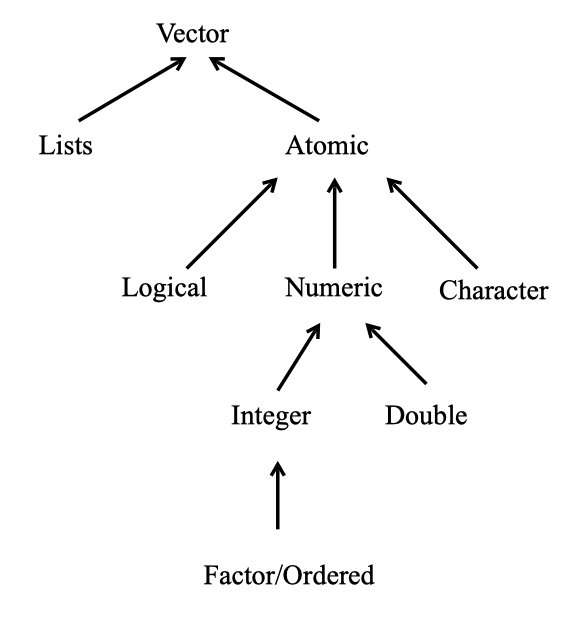
\includegraphics[width=8in]{images/Vector_chart} \end{center}

\hypertarget{additional-resources-1}{%
\section*{Additional Resources}\label{additional-resources-1}}
\addcontentsline{toc}{section}{Additional Resources}

\begin{itemize}
\tightlist
\item
  Chapters 2, 3, 4.1, 4.3, 5.1-5.3, 6 of \href{https://cran.r-project.org/doc/manuals/r-release/R-intro.pdf}{CRAN Intro-to-R Manual}
\item
  Videos:

  \begin{itemize}
  \tightlist
  \item
    \href{https://ucr.yuja.com/V/Video?v=2368642\&node=8487537\&a=1529691043\&autoplay=1}{Variables 1 \textbar{} Types and Assignments}
  \item
    \href{https://ucr.yuja.com/V/Video?v=2368641\&node=8487536\&a=957339369\&autoplay=1}{Variables 2 \textbar{} Nameing Conventions and Best Practices}
  \item
    \href{https://ucr.yuja.com/V/Video?v=2368859\&node=8488053\&a=283774152\&autoplay=1}{Vectors 1 \textbar{} Introduction}
  \end{itemize}
\end{itemize}

\hypertarget{factors-and-lists}{%
\chapter{Factors and Lists}\label{factors-and-lists}}

Factor objects and lists are vectors with special properties. Factors and lists are vectors because they a 1-dimensional sequence of elements. Factors are primarily used for categorical data, and are technically a special form of an integer type vector. However, we will simply refer to a factor vector a as a factor object. Lists are vectors where type of each element can differ. In this chapter we introduce some of the unique properties of factors and lists.

\hypertarget{factors}{%
\section{Factors}\label{factors}}

In real-world problems, you often encounter data that can be classified in categories. For example, suppose a survey was conducted of a group of seven individuals, who were asked to identify their hair color and if they own a pet.

\begin{Shaded}
\begin{Highlighting}[]
\NormalTok{hair =}\StringTok{ }\KeywordTok{c}\NormalTok{(}\StringTok{"Blonde"}\NormalTok{, }\StringTok{"Black"}\NormalTok{, }\StringTok{"Black"}\NormalTok{, }\StringTok{"Red"}\NormalTok{, }\StringTok{"Blonde"}\NormalTok{, }\StringTok{"Brown"}\NormalTok{, }\StringTok{"Black"}\NormalTok{)}
\end{Highlighting}
\end{Shaded}

Here, the hair color and pet ownership are examples of categorical data. For the hair color variable we will typically want to store it as a factor, as opposed to a character vector. The different values that the factor can take are called levels. In R, you can create a factor with the \texttt{factor()}, or the \texttt{as.factor()} functions.

\begin{Shaded}
\begin{Highlighting}[]
\NormalTok{f =}\StringTok{ }\KeywordTok{factor}\NormalTok{(hair)}
\NormalTok{f}
\end{Highlighting}
\end{Shaded}

\begin{verbatim}
## [1] Blonde Black  Black  Red    Blonde Brown  Black 
## Levels: Black Blonde Brown Red
\end{verbatim}

\hypertarget{levels}{%
\subsection{Levels}\label{levels}}

Levels are one of the special properties of a factor object. Notice that when you print the factor, R displays the distinct levels below the factor. R keeps track of all the possible values in a vector, and each value is called a level of the associated factor. The \texttt{levels()} function shows all the levels from a factor.

\begin{Shaded}
\begin{Highlighting}[]
\KeywordTok{levels}\NormalTok{(f)}
\end{Highlighting}
\end{Shaded}

\begin{verbatim}
## [1] "Black"  "Blonde" "Brown"  "Red"
\end{verbatim}

If your vector contains only a subset of all the possible levels, then R will have an incomplete picture of the possible levels. Consider the following example of a vector consisting of directions. Notice that ``South'' is noticeably missing.

\begin{Shaded}
\begin{Highlighting}[]
\NormalTok{directions =}\StringTok{ }\KeywordTok{c}\NormalTok{(}\StringTok{"North"}\NormalTok{, }\StringTok{"West"}\NormalTok{, }\StringTok{"North"}\NormalTok{, }\StringTok{"East"}\NormalTok{, }\StringTok{"North"}\NormalTok{, }\StringTok{"West"}\NormalTok{, }\StringTok{"East"}\NormalTok{)}
\NormalTok{f =}\StringTok{ }\KeywordTok{factor}\NormalTok{(directions)}
\NormalTok{f}
\end{Highlighting}
\end{Shaded}

\begin{verbatim}
## [1] North West  North East  North West  East 
## Levels: East North West
\end{verbatim}

Notice that the levels of your new factor do not contain the value ``South''. R thinks that North, West, and East are the only possible levels. However, in practice, it makes sense to have all the possible directions as levels of your factor. To add all the possible levels explicitly, you specify the \texttt{levels} argument of the function \texttt{factor()}.

\begin{Shaded}
\begin{Highlighting}[]
\NormalTok{directions =}\StringTok{ }\KeywordTok{c}\NormalTok{(}\StringTok{"North"}\NormalTok{, }\StringTok{"West"}\NormalTok{, }\StringTok{"North"}\NormalTok{, }\StringTok{"East"}\NormalTok{, }\StringTok{"North"}\NormalTok{, }\StringTok{"West"}\NormalTok{, }\StringTok{"East"}\NormalTok{)}

\CommentTok{# Make sure all possible categories are listed using the levels argument}
\NormalTok{f =}\StringTok{ }\KeywordTok{factor}\NormalTok{(directions,}
            \DataTypeTok{levels =} \KeywordTok{c}\NormalTok{(}\StringTok{"North"}\NormalTok{, }\StringTok{"East"}\NormalTok{, }\StringTok{"South"}\NormalTok{, }\StringTok{"West"}\NormalTok{))}
\NormalTok{f}
\end{Highlighting}
\end{Shaded}

\begin{verbatim}
## [1] North West  North East  North West  East 
## Levels: North East South West
\end{verbatim}

R lets you assign abbreviated names for the levels. You can do this by specifying the \texttt{labels} argument of \texttt{factor()}.

\begin{Shaded}
\begin{Highlighting}[]
\NormalTok{directions =}\StringTok{ }\KeywordTok{c}\NormalTok{(}\StringTok{"North"}\NormalTok{, }\StringTok{"West"}\NormalTok{, }\StringTok{"South"}\NormalTok{, }\StringTok{"East"}\NormalTok{, }\StringTok{"West"}\NormalTok{, }\StringTok{"North"}\NormalTok{, }\StringTok{"South"}\NormalTok{)}
\NormalTok{f =}\StringTok{ }\KeywordTok{factor}\NormalTok{(directions,}
            \DataTypeTok{levels =} \KeywordTok{c}\NormalTok{(}\StringTok{"North"}\NormalTok{, }\StringTok{"East"}\NormalTok{, }\StringTok{"South"}\NormalTok{, }\StringTok{"West"}\NormalTok{),}
            \DataTypeTok{labels =} \KeywordTok{c}\NormalTok{(}\StringTok{"N"}\NormalTok{, }\StringTok{"E"}\NormalTok{, }\StringTok{"S"}\NormalTok{, }\StringTok{"W"}\NormalTok{))}
\NormalTok{f}
\end{Highlighting}
\end{Shaded}

\begin{verbatim}
## [1] N W S E W N S
## Levels: N E S W
\end{verbatim}

\hypertarget{ordered-factor}{%
\subsection{Ordered Factor}\label{ordered-factor}}

Sometimes data has some kind of natural order between elements. For example, sports analysts use a three-point scale to determine how well a sports team is competing:

\textbf{loss \textless{} tie \textless{} win}.

In market research, it's very common to use a five point scale to measure perceptions:

\textbf{strongly disagree \textless{} disagree \textless{} neutral \textless{} agree \textless{} strongly agree}.

Such kind of data that is possible to place in order or scale is known as \textbf{ordinal data}. We can store ordinal data as an ordered factor. To create an ordered factor, use the \texttt{factor()} function with the argument \texttt{ordered=TRUE}.

\begin{Shaded}
\begin{Highlighting}[]
\NormalTok{record =}\StringTok{ }\KeywordTok{c}\NormalTok{(}\StringTok{"win"}\NormalTok{, }\StringTok{"tie"}\NormalTok{, }\StringTok{"loss"}\NormalTok{, }\StringTok{"tie"}\NormalTok{, }\StringTok{"loss"}\NormalTok{, }\StringTok{"win"}\NormalTok{, }\StringTok{"win"}\NormalTok{)}
\NormalTok{f =}\StringTok{ }\KeywordTok{factor}\NormalTok{(record, }
            \DataTypeTok{ordered =} \OtherTok{TRUE}\NormalTok{)}
\NormalTok{f}
\end{Highlighting}
\end{Shaded}

\begin{verbatim}
## [1] win  tie  loss tie  loss win  win 
## Levels: loss < tie < win
\end{verbatim}

You can manually change which levels are lower and higher based on the order that the levels are listed.

\begin{Shaded}
\begin{Highlighting}[]
\NormalTok{record =}\StringTok{ }\KeywordTok{c}\NormalTok{(}\StringTok{"win"}\NormalTok{, }\StringTok{"tie"}\NormalTok{, }\StringTok{"loss"}\NormalTok{, }\StringTok{"tie"}\NormalTok{, }\StringTok{"loss"}\NormalTok{, }\StringTok{"win"}\NormalTok{, }\StringTok{"win"}\NormalTok{)}
\NormalTok{f =}\StringTok{ }\KeywordTok{factor}\NormalTok{(record, }
           \DataTypeTok{ordered =} \OtherTok{TRUE}\NormalTok{, }
           \DataTypeTok{levels =} \KeywordTok{c}\NormalTok{(}\StringTok{"win"}\NormalTok{, }\StringTok{"tie"}\NormalTok{, }\StringTok{"loss"}\NormalTok{))}
\NormalTok{f}
\end{Highlighting}
\end{Shaded}

\begin{verbatim}
## [1] win  tie  loss tie  loss win  win 
## Levels: win < tie < loss
\end{verbatim}

If you have no observations in one of the levels, you can drop it using the \texttt{droplevels()} function.

\begin{Shaded}
\begin{Highlighting}[]
\NormalTok{record =}\StringTok{ }\KeywordTok{c}\NormalTok{(}\StringTok{"win"}\NormalTok{, }\StringTok{"loss"}\NormalTok{, }\StringTok{"loss"}\NormalTok{, }\StringTok{"win"}\NormalTok{, }\StringTok{"loss"}\NormalTok{, }\StringTok{"win"}\NormalTok{)}
\NormalTok{f =}\StringTok{ }\KeywordTok{factor}\NormalTok{(record,}
           \DataTypeTok{levels =} \KeywordTok{c}\NormalTok{(}\StringTok{"loss"}\NormalTok{, }\StringTok{"tie"}\NormalTok{, }\StringTok{"win"}\NormalTok{))}

\KeywordTok{droplevels}\NormalTok{(f)}
\end{Highlighting}
\end{Shaded}

\begin{verbatim}
## [1] win  loss loss win  loss win 
## Levels: loss win
\end{verbatim}

\hypertarget{factors---basic-features}{%
\section{Factors - Basic Features}\label{factors---basic-features}}

\hypertarget{length-1}{%
\subsection{Length}\label{length-1}}

Factor objects have a lot of the same features as atomic vectors. In general, most of the features and functions we had for atomic vectors work with factors. For example, we still use the \texttt{length()} function to see how many elements are in a factor.

\begin{Shaded}
\begin{Highlighting}[]
\NormalTok{record <-}\StringTok{ }\KeywordTok{c}\NormalTok{(}\StringTok{"win"}\NormalTok{, }\StringTok{"loss"}\NormalTok{, }\StringTok{"loss"}\NormalTok{, }\StringTok{"win"}\NormalTok{, }\StringTok{"loss"}\NormalTok{, }\StringTok{"win"}\NormalTok{)}
\NormalTok{f <-}\StringTok{ }\KeywordTok{factor}\NormalTok{(record)}

\KeywordTok{length}\NormalTok{(f)}
\end{Highlighting}
\end{Shaded}

\begin{verbatim}
## [1] 6
\end{verbatim}

\hypertarget{coercion-1}{%
\subsection{Coercion}\label{coercion-1}}

Coercion also works similarly. We can use \texttt{as.factor()} to create a factor object from a pre-existing vector. As we have seen in the previous examples, the \texttt{factor()} function also works.

\begin{Shaded}
\begin{Highlighting}[]
\NormalTok{record <-}\StringTok{ }\KeywordTok{c}\NormalTok{(}\StringTok{"win"}\NormalTok{, }\StringTok{"loss"}\NormalTok{, }\StringTok{"loss"}\NormalTok{, }\StringTok{"win"}\NormalTok{, }\StringTok{"loss"}\NormalTok{, }\StringTok{"win"}\NormalTok{)}
\NormalTok{f <-}\StringTok{ }\KeywordTok{as.factor}\NormalTok{(record)}
\NormalTok{f}
\end{Highlighting}
\end{Shaded}

\begin{verbatim}
## [1] win  loss loss win  loss win 
## Levels: loss win
\end{verbatim}

To convert a factor object to a non-factor object we still use the \texttt{as.*()} function. In general, it is usually easiest to convert character vectors to factor vectors, and vice versa. When we convert a factor to an integer or double vector the different levels of the factor are converted to integers in order for each level. That is, the first level listed is converted to a 1, the second level listed is converted to a 2, and so on.

\begin{Shaded}
\begin{Highlighting}[]
\CommentTok{# Convert to a character vector }
\KeywordTok{as.character}\NormalTok{(f)}
\end{Highlighting}
\end{Shaded}

\begin{verbatim}
## [1] "win"  "loss" "loss" "win"  "loss" "win"
\end{verbatim}

\begin{Shaded}
\begin{Highlighting}[]
\CommentTok{# Convert to an integer vector }
\KeywordTok{as.integer}\NormalTok{(f)}
\end{Highlighting}
\end{Shaded}

\begin{verbatim}
## [1] 2 1 1 2 1 2
\end{verbatim}

\hypertarget{testingclass}{%
\subsection{Testing/Class}\label{testingclass}}

We can also test if we have factor or an ordered factor using \texttt{is.*()} as we did before.

\begin{Shaded}
\begin{Highlighting}[]
\NormalTok{record =}\StringTok{ }\KeywordTok{c}\NormalTok{(}\StringTok{"win"}\NormalTok{, }\StringTok{"loss"}\NormalTok{, }\StringTok{"loss"}\NormalTok{, }\StringTok{"win"}\NormalTok{, }\StringTok{"loss"}\NormalTok{, }\StringTok{"win"}\NormalTok{)}
\NormalTok{f =}\StringTok{ }\KeywordTok{factor}\NormalTok{(record, }\DataTypeTok{ordered =}\NormalTok{ T)}


\CommentTok{# Test if the character vector is a factor}
\KeywordTok{is.factor}\NormalTok{(record)}
\end{Highlighting}
\end{Shaded}

\begin{verbatim}
## [1] FALSE
\end{verbatim}

\begin{Shaded}
\begin{Highlighting}[]
\CommentTok{# Test if we have a factor (includes both ordered and not ordered factors)}
\KeywordTok{is.factor}\NormalTok{(f)}
\end{Highlighting}
\end{Shaded}

\begin{verbatim}
## [1] TRUE
\end{verbatim}

\begin{Shaded}
\begin{Highlighting}[]
\CommentTok{# Test if we have an ordered factor (only includes ordered factors)}
\KeywordTok{is.ordered}\NormalTok{(f)}
\end{Highlighting}
\end{Shaded}

\begin{verbatim}
## [1] TRUE
\end{verbatim}

With all types of objects we can use the \texttt{class()} function. As mentioned in the previous section, this function returns the name of the type of object that you have, unlike \texttt{typeof()} which returns the storage mode. The output of \texttt{class()} returns name of a object with particular properties. For instance, a factor object. A factor object is stored like an integer vector but it has ``levels'' which can be utilized in special ways.

\begin{Shaded}
\begin{Highlighting}[]
\CommentTok{# Returns storage mode (not recommended)}
\KeywordTok{typeof}\NormalTok{(f)}
\end{Highlighting}
\end{Shaded}

\begin{verbatim}
## [1] "integer"
\end{verbatim}

\begin{Shaded}
\begin{Highlighting}[]
\CommentTok{# Returns class, which is the name of a collection of objects with similar properties }
\CommentTok{# (Recommended)}
\KeywordTok{class}\NormalTok{(f)}
\end{Highlighting}
\end{Shaded}

\begin{verbatim}
## [1] "ordered" "factor"
\end{verbatim}

\hypertarget{names-1}{%
\subsection{Names}\label{names-1}}

Like standard vectors, we can name the elements in a factor using the same three techniques discussed in \ref{names}.

\begin{Shaded}
\begin{Highlighting}[]
\CommentTok{# Using Technique 1 for creating a named vector. }
\NormalTok{named1 <-}\StringTok{ }\KeywordTok{c}\NormalTok{(}\DataTypeTok{sally =} \StringTok{"win"}\NormalTok{, }\DataTypeTok{tom =} \StringTok{"win"}\NormalTok{, }\DataTypeTok{ed =} \StringTok{"lost"}\NormalTok{, }\DataTypeTok{jane =} \StringTok{"tie"}\NormalTok{)}
\NormalTok{named1 <-}\StringTok{ }\KeywordTok{factor}\NormalTok{(named1)}
\NormalTok{named1}
\end{Highlighting}
\end{Shaded}

\begin{verbatim}
## sally   tom    ed  jane 
##   win   win  lost   tie 
## Levels: lost tie win
\end{verbatim}

\hypertarget{accessing-elements}{%
\subsection{Accessing Elements}\label{accessing-elements}}

We can also access elements of a factor object using the same standard techniques described for accessing elements in a vector \ref{index}.

\begin{Shaded}
\begin{Highlighting}[]
\CommentTok{# Obtain the first element}
\NormalTok{named1[}\DecValTok{1}\NormalTok{]}
\end{Highlighting}
\end{Shaded}

\begin{verbatim}
## sally 
##   win 
## Levels: lost tie win
\end{verbatim}

\begin{Shaded}
\begin{Highlighting}[]
\CommentTok{# Obtain the forth and second elements}
\NormalTok{named1[}\KeywordTok{c}\NormalTok{(}\DecValTok{4}\NormalTok{, }\DecValTok{2}\NormalTok{)]}
\end{Highlighting}
\end{Shaded}

\begin{verbatim}
## jane  tom 
##  tie  win 
## Levels: lost tie win
\end{verbatim}

\hypertarget{frequency-tables}{%
\subsection{Frequency Tables}\label{frequency-tables}}

The \texttt{summary()} function will give you a quick overview of the contents of a factor.

\begin{Shaded}
\begin{Highlighting}[]
\NormalTok{hair <-}\StringTok{ }\KeywordTok{c}\NormalTok{(}\StringTok{"Blonde"}\NormalTok{, }\StringTok{"Black"}\NormalTok{, }\StringTok{"Black"}\NormalTok{, }\StringTok{"Red"}\NormalTok{, }\StringTok{"Blonde"}\NormalTok{, }\StringTok{"Brown"}\NormalTok{, }\StringTok{"Black"}\NormalTok{)}
\NormalTok{hair <-}\StringTok{ }\KeywordTok{factor}\NormalTok{(hair)}
\KeywordTok{summary}\NormalTok{(hair)}
\end{Highlighting}
\end{Shaded}

\begin{verbatim}
##  Black Blonde  Brown    Red 
##      3      2      1      1
\end{verbatim}

The function \texttt{table()} tabulates observations.

\begin{Shaded}
\begin{Highlighting}[]
\KeywordTok{table}\NormalTok{(hair)}
\end{Highlighting}
\end{Shaded}

\begin{verbatim}
## hair
##  Black Blonde  Brown    Red 
##      3      2      1      1
\end{verbatim}

We can also use the \texttt{table()} and \texttt{summary()} functions on atomic vectors, and they will operate in a similar way. However, these functions are particularly utilized for factor objects.

The \texttt{table()} function can also tabulate two-way frequency tables.

\begin{Shaded}
\begin{Highlighting}[]
\NormalTok{hair <-}\StringTok{ }\KeywordTok{c}\NormalTok{(}\StringTok{"Blonde"}\NormalTok{, }\StringTok{"Black"}\NormalTok{, }\StringTok{"Black"}\NormalTok{, }\StringTok{"Red"}\NormalTok{, }\StringTok{"Blonde"}\NormalTok{, }\StringTok{"Brown"}\NormalTok{, }\StringTok{"Black"}\NormalTok{)}
\NormalTok{own_pets <-}\StringTok{ }\KeywordTok{c}\NormalTok{(}\OtherTok{TRUE}\NormalTok{, }\OtherTok{FALSE}\NormalTok{, }\OtherTok{TRUE}\NormalTok{, }\OtherTok{TRUE}\NormalTok{, }\OtherTok{FALSE}\NormalTok{, }\OtherTok{FALSE}\NormalTok{, }\OtherTok{FALSE}\NormalTok{)}

\NormalTok{hair <-}\StringTok{ }\KeywordTok{factor}\NormalTok{(hair)}
\NormalTok{own_pets <-}\StringTok{ }\KeywordTok{factor}\NormalTok{(own_pets)}

\KeywordTok{table}\NormalTok{(hair, own_pets)}
\end{Highlighting}
\end{Shaded}

\begin{verbatim}
##         own_pets
## hair     FALSE TRUE
##   Black      2    1
##   Blonde     1    1
##   Brown      1    0
##   Red        0    1
\end{verbatim}

\hypertarget{lists}{%
\section{Lists}\label{lists}}

A \emph{list} is an array of objects. Unlike other types of vectors, the elements in a list can belong to different classes. Lists are useful for packaging together a set of related objects. We can create a list of objects in our environment by using the \texttt{list()} function.

\begin{Shaded}
\begin{Highlighting}[]
\CommentTok{# A list of mixed datatypes}
\NormalTok{lst =}\StringTok{ }\KeywordTok{list}\NormalTok{(1L, }\KeywordTok{c}\NormalTok{(}\StringTok{"abc"}\NormalTok{, }\StringTok{"ABC"}\NormalTok{), }\FloatTok{1.23}\NormalTok{, }\OtherTok{TRUE}\NormalTok{)}
\NormalTok{lst}
\end{Highlighting}
\end{Shaded}

\begin{verbatim}
## [[1]]
## [1] 1
## 
## [[2]]
## [1] "abc" "ABC"
## 
## [[3]]
## [1] 1.23
## 
## [[4]]
## [1] TRUE
\end{verbatim}

Looking at the output above we can see that this output is structured differently than a standard vector. The location of each element of a list is denoted by {[}{[}{]}{]} instead of {[}{]}.

The best way to understand the contents of a list is to use the structure function \texttt{str()}. It provides a compact display of the internal structure of a list.

\begin{Shaded}
\begin{Highlighting}[]
\NormalTok{lst =}\StringTok{ }\KeywordTok{list}\NormalTok{(}\DecValTok{1}\NormalTok{, }\KeywordTok{c}\NormalTok{(}\StringTok{"abc"}\NormalTok{, }\StringTok{"ABC"}\NormalTok{), }\FloatTok{1.23}\NormalTok{, }\OtherTok{TRUE}\NormalTok{)}
\KeywordTok{str}\NormalTok{(lst)}
\end{Highlighting}
\end{Shaded}

\begin{verbatim}
## List of 4
##  $ : num 1
##  $ : chr [1:2] "abc" "ABC"
##  $ : num 1.23
##  $ : logi TRUE
\end{verbatim}

Above we see that we have a list with 4 elements. The first element is of class ``numeric'' and contains a single number, 1. The second element is of ``character'' and contains two elements, which is indicated by {[}1:2{]}. The third and fourth elements are of class ``numeric'' and ``logical'', and each contain a single element.

To see the class of each indivdiual element of a list we can use the following command.

\begin{Shaded}
\begin{Highlighting}[]
\KeywordTok{sapply}\NormalTok{(lst, class)}
\end{Highlighting}
\end{Shaded}

\begin{verbatim}
## [1] "numeric"   "character" "numeric"   "logical"
\end{verbatim}

\hypertarget{nested-lists}{%
\subsection{Nested Lists}\label{nested-lists}}

A list can contain sublists, which in turn can contain sublists themselves, and so on. This is known as \emph{nested list} or \emph{recursive vectors}.

\begin{Shaded}
\begin{Highlighting}[]
\NormalTok{lst =}\StringTok{ }\KeywordTok{list}\NormalTok{(}\DecValTok{1}\NormalTok{, }\DecValTok{3}\NormalTok{, }\KeywordTok{c}\NormalTok{(}\StringTok{"abc"}\NormalTok{, }\StringTok{"ABC"}\NormalTok{), }\KeywordTok{list}\NormalTok{(}\StringTok{"a"}\NormalTok{,}\StringTok{"b"}\NormalTok{,}\StringTok{"c"}\NormalTok{), }\OtherTok{TRUE}\NormalTok{)}
\KeywordTok{str}\NormalTok{(lst)}
\end{Highlighting}
\end{Shaded}

\begin{verbatim}
## List of 5
##  $ : num 1
##  $ : num 3
##  $ : chr [1:2] "abc" "ABC"
##  $ :List of 3
##   ..$ : chr "a"
##   ..$ : chr "b"
##   ..$ : chr "c"
##  $ : logi TRUE
\end{verbatim}

\hypertarget{list---basic-features}{%
\section{List - Basic Features}\label{list---basic-features}}

\hypertarget{length-2}{%
\subsection{Length}\label{length-2}}

Despite looking different and being stored differently than atomic vectors and factors, lists have many of the same properties and features. For example, we still can use the \texttt{length()} function to determine how many elements are in a list.

\begin{Shaded}
\begin{Highlighting}[]
\NormalTok{lst =}\StringTok{ }\KeywordTok{list}\NormalTok{(}\DecValTok{1}\NormalTok{, }\DecValTok{3}\NormalTok{, }\KeywordTok{c}\NormalTok{(}\StringTok{"abc"}\NormalTok{, }\StringTok{"ABC"}\NormalTok{), }\KeywordTok{list}\NormalTok{(}\StringTok{"a"}\NormalTok{,}\StringTok{"b"}\NormalTok{,}\StringTok{"c"}\NormalTok{), }\OtherTok{TRUE}\NormalTok{)}
\KeywordTok{length}\NormalTok{(lst)}
\end{Highlighting}
\end{Shaded}

\begin{verbatim}
## [1] 5
\end{verbatim}

In the example of both there are 5 items in a list. The first two elements are double vectors of length 1, the third element is a character vector of length two, the fourth element is a list of length three, and the fifth element is a logical vector of length 1.
Add elements to a list using \texttt{c()} as we did before with atomic vectors.

\begin{Shaded}
\begin{Highlighting}[]
\NormalTok{lst_char <-}\StringTok{  }\KeywordTok{list}\NormalTok{(}\StringTok{"a"}\NormalTok{, }\StringTok{"b"}\NormalTok{, }\StringTok{"c"}\NormalTok{)}
\NormalTok{lst_num <-}\StringTok{ }\KeywordTok{list}\NormalTok{(}\DecValTok{100}\NormalTok{, }\DecValTok{99}\NormalTok{, }\DecValTok{0}\NormalTok{)}
\NormalTok{lst <-}\StringTok{ }\KeywordTok{c}\NormalTok{(lst_num, lst_char)}
\KeywordTok{str}\NormalTok{(lst)}
\end{Highlighting}
\end{Shaded}

\begin{verbatim}
## List of 6
##  $ : num 100
##  $ : num 99
##  $ : num 0
##  $ : chr "a"
##  $ : chr "b"
##  $ : chr "c"
\end{verbatim}

\hypertarget{coercion-2}{%
\subsection{Coercion}\label{coercion-2}}

We can convert atomic vectors and factors into lists by simply using the \texttt{as.list()} function. The \texttt{as.list()} function lets each element in a vector correspond to each element in the list. So the first element of the vector becomes the first element of the list, the second element of the vector becomes the second element of the list, and so on. We could also use the \texttt{list()} function but this will convert a vector into a list in a different way.

\begin{Shaded}
\begin{Highlighting}[]
\NormalTok{num_vec <-}\StringTok{ }\KeywordTok{c}\NormalTok{(}\DecValTok{1}\NormalTok{, }\DecValTok{2}\NormalTok{, }\DecValTok{3}\NormalTok{)}
\NormalTok{num_lst <-}\StringTok{ }\KeywordTok{as.list}\NormalTok{(num_vec)}
\KeywordTok{str}\NormalTok{(num_lst)}
\end{Highlighting}
\end{Shaded}

\begin{verbatim}
## List of 3
##  $ : num 1
##  $ : num 2
##  $ : num 3
\end{verbatim}

We can convert lists to one of the other types of vectors using the \texttt{as.*()} function with the desired vector type as we did earlier. However, if we do not have a desired type in mind we can also use the \texttt{unlist()} function. The \texttt{unlist()} function takes all atomic objects in a list and creates an atomic vector. In this case R will ``guess'' which type of atomic vector you would like.

\begin{Shaded}
\begin{Highlighting}[]
\KeywordTok{unlist}\NormalTok{(num_lst)}
\end{Highlighting}
\end{Shaded}

\begin{verbatim}
## [1] 1 2 3
\end{verbatim}

\hypertarget{testingclass-1}{%
\subsection{Testing/Class}\label{testingclass-1}}

We can determine if an object is a list or not by using \texttt{is.list()} or the \texttt{class()} functions.

\begin{Shaded}
\begin{Highlighting}[]
\KeywordTok{is.list}\NormalTok{(num_lst)}
\end{Highlighting}
\end{Shaded}

\begin{verbatim}
## [1] TRUE
\end{verbatim}

\begin{Shaded}
\begin{Highlighting}[]
\KeywordTok{class}\NormalTok{(num_lst)}
\end{Highlighting}
\end{Shaded}

\begin{verbatim}
## [1] "list"
\end{verbatim}

\hypertarget{names-2}{%
\subsection{Names}\label{names-2}}

Lists can also be named, and often are. It is very common to created named lists because lists can have a mix of different types objects. We can create a named list using all the same techniques that we used for creating named vectors (\ref{names}) . Notice, we do not have to create a name for every element in a list. Below we see the first two elements are named, and the last is not.

\begin{Shaded}
\begin{Highlighting}[]
\NormalTok{lst <-}\StringTok{ }\KeywordTok{list}\NormalTok{(}\DataTypeTok{first =} \StringTok{"Abraham"}\NormalTok{, }\DataTypeTok{last =} \StringTok{"Lincoln"}\NormalTok{, }\DecValTok{1860}\NormalTok{)}
\NormalTok{lst}
\end{Highlighting}
\end{Shaded}

\begin{verbatim}
## $first
## [1] "Abraham"
## 
## $last
## [1] "Lincoln"
## 
## [[3]]
## [1] 1860
\end{verbatim}

\hypertarget{accessing-elements-1}{%
\subsection{Accessing Elements}\label{accessing-elements-1}}

Accessing elements in a list is a little different than accessing elements in a vector. As you may have already noticed, when a list is outputted into our console the elements in the list are denoted by their index number inside of double brackets, i.e.~{[}{[}2{]}{]}. To access this individual element in a list we use double brackets. This isolates that individual element, and the class of this element is no longer a list but the class of the original element.

\begin{Shaded}
\begin{Highlighting}[]
\NormalTok{lst[[}\DecValTok{1}\NormalTok{]]}
\end{Highlighting}
\end{Shaded}

\begin{verbatim}
## [1] "Abraham"
\end{verbatim}

\begin{Shaded}
\begin{Highlighting}[]
\KeywordTok{class}\NormalTok{(lst[[}\DecValTok{1}\NormalTok{]])}
\end{Highlighting}
\end{Shaded}

\begin{verbatim}
## [1] "character"
\end{verbatim}

We can still use single brackets to access elements in a list, but this method of indexing simply subsets the list. That is, it still returns us a list, just a smaller one based on the indices called.

\begin{Shaded}
\begin{Highlighting}[]
\NormalTok{lst[}\DecValTok{1}\NormalTok{]}
\end{Highlighting}
\end{Shaded}

\begin{verbatim}
## $first
## [1] "Abraham"
\end{verbatim}

\begin{Shaded}
\begin{Highlighting}[]
\KeywordTok{class}\NormalTok{(lst[}\DecValTok{1}\NormalTok{])}
\end{Highlighting}
\end{Shaded}

\begin{verbatim}
## [1] "list"
\end{verbatim}

\begin{Shaded}
\begin{Highlighting}[]
\NormalTok{lst =}\StringTok{ }\KeywordTok{list}\NormalTok{(}\DecValTok{1}\NormalTok{, }\DecValTok{3}\NormalTok{, }\KeywordTok{c}\NormalTok{(}\StringTok{"abc"}\NormalTok{, }\StringTok{"ABC"}\NormalTok{), }\KeywordTok{list}\NormalTok{(}\StringTok{"a"}\NormalTok{,}\StringTok{"b"}\NormalTok{,}\StringTok{"c"}\NormalTok{), }\OtherTok{TRUE}\NormalTok{)}
\NormalTok{lst[}\KeywordTok{c}\NormalTok{(}\DecValTok{3}\NormalTok{, }\DecValTok{1}\NormalTok{)]}
\end{Highlighting}
\end{Shaded}

\begin{verbatim}
## [[1]]
## [1] "abc" "ABC"
## 
## [[2]]
## [1] 1
\end{verbatim}

\begin{Shaded}
\begin{Highlighting}[]
\KeywordTok{class}\NormalTok{(lst[}\KeywordTok{c}\NormalTok{(}\DecValTok{3}\NormalTok{,}\DecValTok{1}\NormalTok{)])}
\end{Highlighting}
\end{Shaded}

\begin{verbatim}
## [1] "list"
\end{verbatim}

\hypertarget{summary-1}{%
\section*{Summary}\label{summary-1}}
\addcontentsline{toc}{section}{Summary}

\begin{itemize}
\item
  Factors are special types of vectors which are primarily used for categorical data.
\item
  Factors can be ordered or unordered.
\item
  We create factor objects using the \texttt{factor()} function.
\item
  Lists are vectors which can have a mix of classes/types of objects.
\item
  We create a factor or list using the functions \texttt{factor()} or \texttt{list()}
\item
  We can use the same basic functions with factors and lists as we do with atomic vectors: \texttt{length()}, \texttt{as.*()}, \texttt{is.*()}, \texttt{class()}
\item
  We have the same basic properties with factors and lists as we do with atomic vectors:

  \begin{itemize}
  \item
    \texttt{length()} determine how long an object is
  \item
    \texttt{c()} combine two objects of the same class together
  \item
    same naming techniques
  \item
    same indexing strategies
  \end{itemize}
\item
  We can also access individual elements of a list using {[}{[}{]}{]}, which isolates an element and takes it out of the list structure.
\end{itemize}

\hypertarget{matrices-data-frames-and-more}{%
\chapter{Matrices, Data Frames, and More}\label{matrices-data-frames-and-more}}

\hypertarget{matrices}{%
\section{Matrices}\label{matrices}}

A matrix is a two dimensional array of data of \textbf{the same type}. The matrix function, \texttt{matrix()}, can be used to create a new matrix.

\begin{Shaded}
\begin{Highlighting}[]
\NormalTok{m =}\StringTok{ }\KeywordTok{matrix}\NormalTok{(}\KeywordTok{c}\NormalTok{(}\DecValTok{1}\NormalTok{, }\DecValTok{9}\NormalTok{, }\DecValTok{2}\NormalTok{, }\DecValTok{0}\NormalTok{, }\DecValTok{5}\NormalTok{, }\DecValTok{7}\NormalTok{, }\DecValTok{3}\NormalTok{, }\DecValTok{8}\NormalTok{, }\DecValTok{4}\NormalTok{), }
           \DataTypeTok{nrow=}\DecValTok{3}\NormalTok{, }\DataTypeTok{ncol=}\DecValTok{3}\NormalTok{)}
\NormalTok{m}
\end{Highlighting}
\end{Shaded}

\begin{verbatim}
##      [,1] [,2] [,3]
## [1,]    1    0    3
## [2,]    9    5    8
## [3,]    2    7    4
\end{verbatim}

R labels the rows and columns for us in the output. The matrix is filled column-by-column using the elements of the vector created by the concatenate function. The matrix \texttt{m} above is a matrix composed of doubles (the atomic object). This is the default type of matrix R creates, and it is by far the most common matrix used. However, we can also create integer matrices, logical matrices, and character matrices.

\begin{Shaded}
\begin{Highlighting}[]
\CommentTok{# Example of a matrix with logical values}
\NormalTok{m_logical <-}\StringTok{ }\KeywordTok{matrix}\NormalTok{(}\KeywordTok{c}\NormalTok{(T, T, T, F, F, F, T, T), }
                    \DataTypeTok{nrow =} \DecValTok{4}\NormalTok{, }\DataTypeTok{ncol =} \DecValTok{2}\NormalTok{)}
\NormalTok{m_logical }
\end{Highlighting}
\end{Shaded}

\begin{verbatim}
##       [,1]  [,2]
## [1,]  TRUE FALSE
## [2,]  TRUE FALSE
## [3,]  TRUE  TRUE
## [4,] FALSE  TRUE
\end{verbatim}

\hypertarget{vectorized-operations}{%
\subsection{Vectorized Operations}\label{vectorized-operations}}

As with vectors, matrices can be used in arithmetic operations with scalars and other matrices of the same size. We still have all the same basic vectorized operations.

\begin{Shaded}
\begin{Highlighting}[]
\NormalTok{m2 =}\StringTok{ }\NormalTok{m}\OperatorTok{/}\DecValTok{2}
\NormalTok{m2}
\end{Highlighting}
\end{Shaded}

\begin{verbatim}
##      [,1] [,2] [,3]
## [1,]  0.5  0.0  1.5
## [2,]  4.5  2.5  4.0
## [3,]  1.0  3.5  2.0
\end{verbatim}

\begin{Shaded}
\begin{Highlighting}[]
\NormalTok{m }\OperatorTok{*}\NormalTok{m2}
\end{Highlighting}
\end{Shaded}

\begin{verbatim}
##      [,1] [,2] [,3]
## [1,]  0.5  0.0  4.5
## [2,] 40.5 12.5 32.0
## [3,]  2.0 24.5  8.0
\end{verbatim}

\hypertarget{data-frames}{%
\section{Data Frames}\label{data-frames}}

Like a matrix, a data frame is a rectangular array of values where each column is a vector. However, unlike a matrix, the columns can be different data types. We can create a set of vectors of the same length and use the \texttt{data.frame()} function to make a data frame object.

\begin{Shaded}
\begin{Highlighting}[]
\NormalTok{age <-}\StringTok{ }\KeywordTok{c}\NormalTok{(}\DecValTok{1}\NormalTok{, }\DecValTok{8}\NormalTok{, }\DecValTok{10}\NormalTok{, }\DecValTok{30}\NormalTok{, }\DecValTok{31}\NormalTok{)}
\NormalTok{gender <-}\StringTok{ }\KeywordTok{c}\NormalTok{(}\StringTok{"Female"}\NormalTok{, }\StringTok{"Female"}\NormalTok{, }\StringTok{"Male"}\NormalTok{,}\StringTok{"Female"}\NormalTok{,}\StringTok{"Male"}\NormalTok{)}
\NormalTok{married <-}\StringTok{ }\KeywordTok{c}\NormalTok{(}\OtherTok{FALSE}\NormalTok{, }\OtherTok{FALSE}\NormalTok{, }\OtherTok{FALSE}\NormalTok{, }\OtherTok{TRUE}\NormalTok{, }\OtherTok{TRUE}\NormalTok{)}
\NormalTok{simpsons <-}\StringTok{ }\KeywordTok{data.frame}\NormalTok{(age, gender, married)}
\NormalTok{simpsons}
\end{Highlighting}
\end{Shaded}

\begin{verbatim}
##   age gender married
## 1   1 Female   FALSE
## 2   8 Female   FALSE
## 3  10   Male   FALSE
## 4  30 Female    TRUE
## 5  31   Male    TRUE
\end{verbatim}

\begin{Shaded}
\begin{Highlighting}[]
\KeywordTok{class}\NormalTok{(simpsons)}
\end{Highlighting}
\end{Shaded}

\begin{verbatim}
## [1] "data.frame"
\end{verbatim}

To see all the class of each column in a data frame we can use the following command.

\begin{Shaded}
\begin{Highlighting}[]
\KeywordTok{sapply}\NormalTok{(simpsons, class)}
\end{Highlighting}
\end{Shaded}

\begin{verbatim}
##         age      gender     married 
##   "numeric" "character"   "logical"
\end{verbatim}

\hypertarget{column-names}{%
\subsection{Column Names}\label{column-names}}

Data frames always have column names. In the example above we used vectors to create a data frame. When we use this technique then the name of the vector is automatically selected as the column name. If we have inputted a vector like \texttt{c(1,\ 2,\ 3,\ 4,\ 5)} as an argument in the \texttt{data.frame()} function instead of an object name, then R would have guessed what to name the column. Matrices do not have this property. Matrices do not usually have column or row names (but they can, as we will see below). In contrast, data frames always have column names, and often have row names too. In the following section we discuss how to change the row and column names of both matrices and data frames explicitly.

\hypertarget{basic-features-of-matricesdata-frames}{%
\section{Basic Features of Matrices/Data-Frames}\label{basic-features-of-matricesdata-frames}}

\hypertarget{dimensions}{%
\subsection{Dimensions}\label{dimensions}}

To access and determine the size or dimensions of a matrix and data frame there are three important functions. We no longer would want to use the \texttt{length()} function because that is for 1-dimsional objects. Since matrices and data frames are 2-dimensional objects we now must consider both dimensions. The three functions we can use to do this are \texttt{dim()}, \texttt{nrow()}, and \texttt{ncol()}. The \texttt{dim()} function returns the number of rows and the number of columns. The \texttt{nrow()} just returns the number of rows, and \texttt{ncol()} just returns the number of columns.

\begin{Shaded}
\begin{Highlighting}[]
\KeywordTok{dim}\NormalTok{(simpsons)}
\end{Highlighting}
\end{Shaded}

\begin{verbatim}
## [1] 5 3
\end{verbatim}

\begin{Shaded}
\begin{Highlighting}[]
\KeywordTok{nrow}\NormalTok{(simpsons)}
\end{Highlighting}
\end{Shaded}

\begin{verbatim}
## [1] 5
\end{verbatim}

\begin{Shaded}
\begin{Highlighting}[]
\KeywordTok{ncol}\NormalTok{(simpsons)}
\end{Highlighting}
\end{Shaded}

\begin{verbatim}
## [1] 3
\end{verbatim}

\hypertarget{accesing-elements}{%
\subsection{Accesing Elements}\label{accesing-elements}}

Indices can be used to obtain the elements of a matrix and data frame, but now we must consider both the row and column. We can access an individual point in a matrix or data frame using \texttt{{[}row,\ colum{]}}, where \texttt{row} is the row index and \texttt{column} is the column index.

\begin{Shaded}
\begin{Highlighting}[]
\NormalTok{m =}\StringTok{ }\KeywordTok{matrix}\NormalTok{(}\KeywordTok{c}\NormalTok{(}\DecValTok{1}\NormalTok{, }\DecValTok{9}\NormalTok{, }\DecValTok{2}\NormalTok{, }\DecValTok{0}\NormalTok{, }\DecValTok{5}\NormalTok{, }\DecValTok{7}\NormalTok{, }\DecValTok{3}\NormalTok{, }\DecValTok{8}\NormalTok{, }\DecValTok{4}\NormalTok{), }
           \DataTypeTok{nrow=}\DecValTok{3}\NormalTok{, }\DataTypeTok{ncol=}\DecValTok{3}\NormalTok{)}
\NormalTok{m[}\DecValTok{2}\NormalTok{,}\DecValTok{2}\NormalTok{]}
\end{Highlighting}
\end{Shaded}

\begin{verbatim}
## [1] 5
\end{verbatim}

We can access multiple elements using the \texttt{c()} function. Note we must use the \texttt{c()} function to separate the rows and columns we are trying isolate because the common inside the single brackets separates the dimensions.

\begin{Shaded}
\begin{Highlighting}[]
\CommentTok{# Isolate multiple individual points. }
\NormalTok{m[}\KeywordTok{c}\NormalTok{(}\DecValTok{1}\NormalTok{,}\DecValTok{3}\NormalTok{), }\KeywordTok{c}\NormalTok{(}\DecValTok{1}\NormalTok{,}\DecValTok{3}\NormalTok{)]}
\end{Highlighting}
\end{Shaded}

\begin{verbatim}
##      [,1] [,2]
## [1,]    1    3
## [2,]    2    4
\end{verbatim}

We can also isolate entire rows or columns by leaving one of the dimensions blank.

\begin{Shaded}
\begin{Highlighting}[]
\CommentTok{# Isolate the second row}
\NormalTok{m[}\DecValTok{2}\NormalTok{,]}
\end{Highlighting}
\end{Shaded}

\begin{verbatim}
## [1] 9 5 8
\end{verbatim}

\begin{Shaded}
\begin{Highlighting}[]
\CommentTok{# Isolate the third column }
\NormalTok{m[,}\DecValTok{3}\NormalTok{]}
\end{Highlighting}
\end{Shaded}

\begin{verbatim}
## [1] 3 8 4
\end{verbatim}

We can think of these individual rows or columns as an individual vector.

\begin{Shaded}
\begin{Highlighting}[]
\NormalTok{vec =}\StringTok{ }\NormalTok{simpsons[,}\DecValTok{2}\NormalTok{]}
\NormalTok{vec}
\end{Highlighting}
\end{Shaded}

\begin{verbatim}
## [1] "Female" "Female" "Male"   "Female" "Male"
\end{verbatim}

\hypertarget{coercion-3}{%
\subsection{Coercion}\label{coercion-3}}

We often do not need to convert matrices and data frames, but if we do we can use the \texttt{as.matrix()} or \texttt{as.data.frame()} on a pre-existing object to convert it into a matrix or data frame. The most common type of coercion that we have for 2-dimensional objects is changing the class of a column in a data frame. To do this we can redefine this class explicitly using indexing.

\begin{Shaded}
\begin{Highlighting}[]
\CommentTok{# Changing the class of a single column }
\NormalTok{simpsons[, }\DecValTok{1}\NormalTok{] <-}\StringTok{ }\KeywordTok{as.factor}\NormalTok{(simpsons[, }\DecValTok{1}\NormalTok{])}

\KeywordTok{sapply}\NormalTok{(simpsons, class)}
\end{Highlighting}
\end{Shaded}

\begin{verbatim}
##         age      gender     married 
##    "factor" "character"   "logical"
\end{verbatim}

\begin{Shaded}
\begin{Highlighting}[]
\NormalTok{simpsons}
\end{Highlighting}
\end{Shaded}

\begin{verbatim}
##   age gender married
## 1   1 Female   FALSE
## 2   8 Female   FALSE
## 3  10   Male   FALSE
## 4  30 Female    TRUE
## 5  31   Male    TRUE
\end{verbatim}

\hypertarget{testingclass-2}{%
\subsection{Testing/Class}\label{testingclass-2}}

We can test or determine what type of object we have using the \texttt{class()} function. Again, this function will always return something for a given object. If we have a data frame or matrix it will return ``data.frame'' or ``matrix'', respectively. We can also use the \texttt{is.matrix()} or \texttt{is.data.frame()} functions which will return \texttt{TRUE/FALSE} values.

\hypertarget{names-3}{%
\subsection{Names}\label{names-3}}

With both matrices and data frames we can name the rows and columns. Data frames will always have column names, but matrices do not have to have them. It is very commmon to name the rows and columns for a data frame, but not as common for matrices. Matrices are most often used for linear algebra calculations. To see the row or column names of a 2-dimensional object we can use the \texttt{rownames()} and \texttt{colnames()} functions.

\begin{Shaded}
\begin{Highlighting}[]
\KeywordTok{rownames}\NormalTok{(simpsons)}
\end{Highlighting}
\end{Shaded}

\begin{verbatim}
## [1] "1" "2" "3" "4" "5"
\end{verbatim}

\begin{Shaded}
\begin{Highlighting}[]
\KeywordTok{colnames}\NormalTok{(simpsons)}
\end{Highlighting}
\end{Shaded}

\begin{verbatim}
## [1] "age"     "gender"  "married"
\end{verbatim}

To change these names we use the same functions, and just manually reassign the values for them.

\begin{Shaded}
\begin{Highlighting}[]
\KeywordTok{rownames}\NormalTok{(simpsons) <-}\StringTok{ }\KeywordTok{c}\NormalTok{(}\StringTok{"Maggie"}\NormalTok{, }\StringTok{"Lisa"}\NormalTok{, }\StringTok{"Bart"}\NormalTok{, }\StringTok{"Marge"}\NormalTok{, }\StringTok{"Homer"}\NormalTok{)}
\NormalTok{simpsons}
\end{Highlighting}
\end{Shaded}

\begin{verbatim}
##        age gender married
## Maggie   1 Female   FALSE
## Lisa     8 Female   FALSE
## Bart    10   Male   FALSE
## Marge   30 Female    TRUE
## Homer   31   Male    TRUE
\end{verbatim}

\begin{Shaded}
\begin{Highlighting}[]
\KeywordTok{colnames}\NormalTok{(simpsons) <-}\StringTok{ }\KeywordTok{c}\NormalTok{(}\StringTok{"Age"}\NormalTok{, }\StringTok{"Gender"}\NormalTok{, }\StringTok{"Married"}\NormalTok{)}
\NormalTok{simpsons}
\end{Highlighting}
\end{Shaded}

\begin{verbatim}
##        Age Gender Married
## Maggie   1 Female   FALSE
## Lisa     8 Female   FALSE
## Bart    10   Male   FALSE
## Marge   30 Female    TRUE
## Homer   31   Male    TRUE
\end{verbatim}

\hypertarget{other-object-types-and-the-global-environment}{%
\section{Other Object Types and the Global Environment}\label{other-object-types-and-the-global-environment}}

There are more objects then what we have discussed above. For example, many of the advanced functions create specific objects generated by that specific function. There are hundreds, and possibly thousands, of such objects. These objects generally are special cases of lists, factors, and other various types of objects that we have defined in this section. The objects we have described here are the building blocks of most values we will be working with. Functions like \texttt{class()} and \texttt{length()} are also considered as objects, but are of a different type. We discuss functions in more detail in section \ref{functions}.

There are also built-in, or special objects in R. For example, the object \texttt{pi} is an object already defined. These built-in values and functions can be written over, but that is not advised.

\begin{Shaded}
\begin{Highlighting}[]
\NormalTok{pi}
\end{Highlighting}
\end{Shaded}

\begin{verbatim}
## [1] 3.141593
\end{verbatim}

Every time we create an object we see that the Global Environment tab in the top right pane updates. The object we have created is now listed in the Global Environment. This is a collection of all \emph{user created} objects in R, that R knows about, and that R can easily call. Built-in objects, such as \texttt{pi}, will not be listed here.

\hypertarget{summary-2}{%
\section*{Summary}\label{summary-2}}
\addcontentsline{toc}{section}{Summary}

\begin{itemize}
\item
  The basic and most common 2-dimensional objects are matrices and data frames.
\item
  Matrices must contain all data of the same type.
\item
  Data frames can have different classes between columns, and always have column names.
\item
  We can create a matrix or data frame using the \texttt{matrix()} and \texttt{data.frame()} functions.
\item
  Many vectorized operations still work for 2-dimensional objects.
\item
  We can look at and name both rows and columns using \texttt{rownames()} and \texttt{colnames()}.
\item
  To see the dimensions of a 2-dimensional object we use \texttt{dim()}, \texttt{nrow()} and \texttt{ncol()}.
\item
  We can check if we have a matrix or data frame by using \texttt{class()} or \texttt{is.*()}.
\item
  To access elements of a 2-dimsional object we use \texttt{{[}row,\ column{]}}.
\end{itemize}

\hypertarget{indexing}{%
\chapter{Indexing}\label{indexing}}

When we wish to extract elements of an object like a vector, list, data frame, or matrix, we use a process called \emph{indexing}. The process of indexing, is also sometimes called \emph{subsetting}. In R the \emph{index} of an object is the numeric location of that object. For example, consider the vector \texttt{vec\ \textless{}-\ c(100,\ 20,\ 3)}. The index of the first element is 1, the index of the second element is 2, and the so on. We have already seen a few examples of indexing for vectors and factors, lists, and 2D objects. In this section we more formally describe a plethora of indexing techniques. Indexing can be hard to master in R because of the many options, and the different types of objects. In this section we will describe the basic indexing techniques for atomic vector and factors, lists, matrices, and data frames. The indexing between the methods are all related, so it useful to talk about them all together. At the end of this section we give examples of a few features and applications we can do with indexing.

\hypertarget{VectorIndex}{%
\section{Atomic Vectors and Factors}\label{VectorIndex}}

We have already seen a little big of indexing with vectors (atomic, factors, and lists). Now we will discuss indexing in more detail for 1D Objects. We will focus specifically on atomic vectors. The techniques here can be used with other types and classes of vectors though. For indexing with vectors we only have one indexing operator, \texttt{{[}{]}}. We also have four general strategies that we will focus on. Suppose we wish to preform indexing on a vector \texttt{vec}.

\begin{Shaded}
\begin{Highlighting}[]
\CommentTok{# Generate a random vector with the following code }
\KeywordTok{set.seed}\NormalTok{(}\DecValTok{10}\NormalTok{)}
\NormalTok{vec <-}\StringTok{ }\KeywordTok{sample}\NormalTok{(}\DecValTok{1}\OperatorTok{:}\DecValTok{100}\NormalTok{, }\DecValTok{10}\NormalTok{)  }\CommentTok{# numeric vector with 10 values}
\NormalTok{vec}
\end{Highlighting}
\end{Shaded}

\begin{verbatim}
##  [1]  9 74 76 55 72 54 39 83 88 15
\end{verbatim}

\begin{itemize}
\tightlist
\item
  Four basic strategies:

  \begin{itemize}
  \tightlist
  \item
    \textbf{positive integer}: When using the positive integer strategy we use a vector \texttt{index} which only contains positive integers of the indexes. This vector can be of any positive finite length. That means it can be of length 1, length 10, or even length 10000. We use this operator by calling \texttt{vec{[}index{]}}, which will return the elements of \texttt{vec} by their indices as ordered from \texttt{index}.
  \item
    \textbf{negative integer}: The negative integer strategy works similarly. This time we consider a vector \texttt{index} which only contains negative integers, and must have a positive length between 1 and the length of \texttt{vec}. These correspond to the elements of \texttt{vec} you would like to exclude.\\
  \item
    \textbf{logical elements}: When using the logical strategy we use a vector \texttt{index} which contains only logical (\texttt{TRUE/FALSE}) values. In this strategy \texttt{index} must be the same length as the vector \texttt{vec}. If it is not, R will use \emph{recycling} to complete the command. The \texttt{TRUE} values in \texttt{index} represent the elements of \texttt{vec} you wish to keep, and \texttt{FALSE} values represent the elements you wish to exclude.
  \item
    \textbf{names}: If \texttt{vec} is a named vector we can also use the names to preform indexing. In this case the vector \texttt{index} should be a character vector where each element of the vector is the name of an element in \texttt{vec} that we wish to keep. We can not use a negative operator, or a negative sign with this strategy to exclude variables.
  \end{itemize}
\end{itemize}

We can not mix and max these strategies within a command. We can only use one strategy at a time.

\hypertarget{example-positive-integers}{%
\subsection*{Example: Positive Integers}\label{example-positive-integers}}
\addcontentsline{toc}{subsection}{Example: Positive Integers}

\begin{Shaded}
\begin{Highlighting}[]
\CommentTok{# Obtaining a single element }
\NormalTok{vec[}\DecValTok{1}\NormalTok{]}
\end{Highlighting}
\end{Shaded}

\begin{verbatim}
## [1] 9
\end{verbatim}

\begin{Shaded}
\begin{Highlighting}[]
\CommentTok{# Obtaining several elements: Get 1st, 2nd, 3rd element}
\NormalTok{vec[}\KeywordTok{c}\NormalTok{(}\DecValTok{1}\NormalTok{, }\DecValTok{2}\NormalTok{, }\DecValTok{3}\NormalTok{)]}
\end{Highlighting}
\end{Shaded}

\begin{verbatim}
## [1]  9 74 76
\end{verbatim}

\begin{Shaded}
\begin{Highlighting}[]
\CommentTok{# Get mutliples of the same element}
\NormalTok{index <-}\StringTok{ }\KeywordTok{c}\NormalTok{(}\DecValTok{3}\NormalTok{, }\DecValTok{2}\NormalTok{, }\DecValTok{1}\NormalTok{, }\DecValTok{1}\NormalTok{, }\DecValTok{1}\NormalTok{, }\DecValTok{2}\NormalTok{, }\DecValTok{3}\NormalTok{)}
\NormalTok{vec[index]}
\end{Highlighting}
\end{Shaded}

\begin{verbatim}
## [1] 76 74  9  9  9 74 76
\end{verbatim}

\hypertarget{example-negative-integers}{%
\subsection*{Example: Negative Integers}\label{example-negative-integers}}
\addcontentsline{toc}{subsection}{Example: Negative Integers}

\begin{Shaded}
\begin{Highlighting}[]
\CommentTok{# Remove first element}
\NormalTok{vec[}\DecValTok{1}\NormalTok{]}
\end{Highlighting}
\end{Shaded}

\begin{verbatim}
## [1] 9
\end{verbatim}

\begin{Shaded}
\begin{Highlighting}[]
\CommentTok{# Remove several elements: 1st, 2nd, 3rd }
\NormalTok{vec[}\OperatorTok{-}\KeywordTok{c}\NormalTok{(}\DecValTok{1}\NormalTok{, }\DecValTok{2}\NormalTok{, }\DecValTok{3}\NormalTok{)]}
\end{Highlighting}
\end{Shaded}

\begin{verbatim}
## [1] 55 72 54 39 83 88 15
\end{verbatim}

\begin{Shaded}
\begin{Highlighting}[]
\CommentTok{# Equivalent to above }
\NormalTok{index <-}\StringTok{ }\KeywordTok{c}\NormalTok{(}\OperatorTok{-}\DecValTok{1}\NormalTok{, }\DecValTok{-2}\NormalTok{, }\DecValTok{-3}\NormalTok{)}
\NormalTok{vec[index]}
\end{Highlighting}
\end{Shaded}

\begin{verbatim}
## [1] 55 72 54 39 83 88 15
\end{verbatim}

\hypertarget{example-logical-values}{%
\subsection*{Example: Logical Values}\label{example-logical-values}}
\addcontentsline{toc}{subsection}{Example: Logical Values}

\begin{Shaded}
\begin{Highlighting}[]
\CommentTok{# `index` should be the same length as `vec`}
\NormalTok{index <-}\StringTok{ }\KeywordTok{c}\NormalTok{(T, T, T, T, F, }
\NormalTok{           F, F, F, F, T)}
\NormalTok{vec[index]}
\end{Highlighting}
\end{Shaded}

\begin{verbatim}
## [1]  9 74 76 55 15
\end{verbatim}

\begin{Shaded}
\begin{Highlighting}[]
\CommentTok{# When `index` is not of the same length as `vec`, we have recycling}
\CommentTok{# Keeps every other element }
\NormalTok{index <-}\StringTok{ }\KeywordTok{c}\NormalTok{(T, F)}
\NormalTok{vec[index]}
\end{Highlighting}
\end{Shaded}

\begin{verbatim}
## [1]  9 76 72 39 88
\end{verbatim}

\hypertarget{example-names}{%
\subsection*{Example: Names}\label{example-names}}
\addcontentsline{toc}{subsection}{Example: Names}

\begin{Shaded}
\begin{Highlighting}[]
\CommentTok{# Give names to each element in `vec`}
\KeywordTok{names}\NormalTok{(vec) =}\StringTok{ }\NormalTok{LETTERS[}\DecValTok{1}\OperatorTok{:}\DecValTok{10}\NormalTok{]}

\CommentTok{# Return Elements: A, B, D}
\NormalTok{index =}\StringTok{ }\KeywordTok{c}\NormalTok{(}\StringTok{"A"}\NormalTok{, }\StringTok{"B"}\NormalTok{, }\StringTok{"D"}\NormalTok{)}
\NormalTok{vec[index]}
\end{Highlighting}
\end{Shaded}

\begin{verbatim}
##  A  B  D 
##  9 74 55
\end{verbatim}

\hypertarget{lists-1}{%
\section{Lists}\label{lists-1}}

Although lists are 1D objects, they have three different operators: \texttt{{[}{]}}, \texttt{{[}{[}{]}{]}}, and \texttt{\$}. The first operator works the same way as we saw above for atomic vectors. We can use all four strategies we used in the prior section, and a new list will appear according to the indexing order. The new operators are \texttt{{[}{[}{]}{]}} and \texttt{\$}, these operators are very similar. They both can only isolate one element in the list, and they return this element in its particular class. That is, if the second element in the list is data frame, then a data frame is returned with the \texttt{{[}{[}{]}{]}} and \texttt{\$} operators.

\hypertarget{double-brackets}{%
\subsection{Double Brackets}\label{double-brackets}}

With the double brackets operator \texttt{{[}{[}index{]}{]}} we can put the index number for the element we want returned, or if we have a named list, we can put the name of the element we desire. Remember, you can only isolate one element in the list using this operator, so \texttt{index} must be of length 1.

\begin{Shaded}
\begin{Highlighting}[]
\CommentTok{# Create a named list}
\CommentTok{# Recall: name = value }
\NormalTok{lst1 =}\StringTok{ }\KeywordTok{list}\NormalTok{(}\DataTypeTok{first =} \KeywordTok{c}\NormalTok{(}\StringTok{"Hello"}\NormalTok{, }\StringTok{"Goodbye"}\NormalTok{), }\DataTypeTok{second =} \KeywordTok{c}\NormalTok{(}\DecValTok{1}\NormalTok{, }\DecValTok{2}\NormalTok{, }\DecValTok{3}\NormalTok{), }\DataTypeTok{third =} \KeywordTok{c}\NormalTok{(T, F, T))}

\CommentTok{# Create a nested list with names }
\NormalTok{lst2 =}\StringTok{ }\KeywordTok{list}\NormalTok{(}\DataTypeTok{e1 =}\NormalTok{ lst1, }\DataTypeTok{e2 =} \StringTok{"Stat 107 Rules"}\NormalTok{)}

\CommentTok{# See structure of the list }
\KeywordTok{str}\NormalTok{(lst2)}
\end{Highlighting}
\end{Shaded}

\begin{verbatim}
## List of 2
##  $ e1:List of 3
##   ..$ first : chr [1:2] "Hello" "Goodbye"
##   ..$ second: num [1:3] 1 2 3
##   ..$ third : logi [1:3] TRUE FALSE TRUE
##  $ e2: chr "Stat 107 Rules"
\end{verbatim}

\begin{Shaded}
\begin{Highlighting}[]
\CommentTok{# Isolate second element by name (maintains class of the element)}
\NormalTok{lst2[[}\StringTok{"e2"}\NormalTok{]]}
\end{Highlighting}
\end{Shaded}

\begin{verbatim}
## [1] "Stat 107 Rules"
\end{verbatim}

\begin{Shaded}
\begin{Highlighting}[]
\KeywordTok{class}\NormalTok{(lst2[[}\StringTok{"e2"}\NormalTok{]])}
\end{Highlighting}
\end{Shaded}

\begin{verbatim}
## [1] "character"
\end{verbatim}

\begin{Shaded}
\begin{Highlighting}[]
\CommentTok{# Isolate second element by integer (maintains class of the element) }
\NormalTok{lst2[[}\DecValTok{2}\NormalTok{]]}
\end{Highlighting}
\end{Shaded}

\begin{verbatim}
## [1] "Stat 107 Rules"
\end{verbatim}

\begin{Shaded}
\begin{Highlighting}[]
\KeywordTok{class}\NormalTok{(lst2[[}\DecValTok{2}\NormalTok{]])}
\end{Highlighting}
\end{Shaded}

\begin{verbatim}
## [1] "character"
\end{verbatim}

\begin{Shaded}
\begin{Highlighting}[]
\CommentTok{# Isolate nested elements}
\NormalTok{lst2[[}\DecValTok{1}\NormalTok{]][[}\DecValTok{2}\NormalTok{]]}
\end{Highlighting}
\end{Shaded}

\begin{verbatim}
## [1] 1 2 3
\end{verbatim}

\hypertarget{dollar-sign}{%
\subsection{Dollar Sign}\label{dollar-sign}}

After the dollar sign operator \texttt{\$} we put the name of the desired element. You can only isolate one element in the list using this operator, and you can only access elements using their names. However, if you have

\begin{Shaded}
\begin{Highlighting}[]
\CommentTok{# Isolate second element by name (maintains class of the element)}
\NormalTok{lst2}\OperatorTok{$}\NormalTok{e2}
\end{Highlighting}
\end{Shaded}

\begin{verbatim}
## [1] "Stat 107 Rules"
\end{verbatim}

\begin{Shaded}
\begin{Highlighting}[]
\CommentTok{# Isolate nested elements}
\NormalTok{lst2}\OperatorTok{$}\NormalTok{e1}\OperatorTok{$}\NormalTok{second}
\end{Highlighting}
\end{Shaded}

\begin{verbatim}
## [1] 1 2 3
\end{verbatim}

You can also mix and match indexing methods for lists.

\begin{Shaded}
\begin{Highlighting}[]
\NormalTok{lst1}\OperatorTok{$}\NormalTok{second[}\DecValTok{2}\NormalTok{]}
\end{Highlighting}
\end{Shaded}

\begin{verbatim}
## [1] 2
\end{verbatim}

\hypertarget{matrices-1}{%
\section{Matrices}\label{matrices-1}}

For matrices we will only consider three indexing techniques, these are by far the most popular. There is only one operator we need to consider for matrices, and it is the same one we use for vectors \texttt{{[}{]}}. Inside this operator you can put in two vectors, or a single vector.

\hypertarget{two-vectors}{%
\subsection{Two Vectors}\label{two-vectors}}

Using two vectors when indexing a list is by far the most common, and the recommended way to index a matrix. It is easy to read, and standard practice. For this technique you use \texttt{{[}row,\ column{]}}, where \texttt{row} is a vector of index values of the rows you wish to isolate, and \texttt{column} is a vector of the index values of the columns you wish to isolate. The vectors \texttt{row} and \texttt{column} support positive integers, negative integers, logical vectors, and character vectors with row and column names. That is, we can index the rows and columns of a matrix in the same way we did before with standard vectors, but now we have two dimensions to consider. Like before, the vectors \texttt{row} and \texttt{column} must be all positive values, all negative values, all logical, or only contain the respective names. However, the values between vectors can differ. For example, \texttt{row} can be a vector of positive integers, and \texttt{column} can be a vector of logical values. In general, a matrix returns another matrix, or it returns a vector.

\begin{Shaded}
\begin{Highlighting}[]
\NormalTok{my_m =}\StringTok{ }\KeywordTok{matrix}\NormalTok{(}\DecValTok{1}\OperatorTok{:}\DecValTok{9}\NormalTok{, }\DataTypeTok{nrow =} \DecValTok{3}\NormalTok{, }\DataTypeTok{ncol =} \DecValTok{3}\NormalTok{)}
\KeywordTok{colnames}\NormalTok{(my_m) =}\StringTok{ }\KeywordTok{c}\NormalTok{(}\StringTok{"C1"}\NormalTok{, }\StringTok{"C2"}\NormalTok{, }\StringTok{"C3"}\NormalTok{)}
\NormalTok{my_m}
\end{Highlighting}
\end{Shaded}

\begin{verbatim}
##      C1 C2 C3
## [1,]  1  4  7
## [2,]  2  5  8
## [3,]  3  6  9
\end{verbatim}

\begin{Shaded}
\begin{Highlighting}[]
\CommentTok{# Obtain a full row }
\NormalTok{my_m[}\DecValTok{1}\NormalTok{,]}
\end{Highlighting}
\end{Shaded}

\begin{verbatim}
## C1 C2 C3 
##  1  4  7
\end{verbatim}

\begin{Shaded}
\begin{Highlighting}[]
\CommentTok{# Obtain a full column }
\NormalTok{my_m[,}\DecValTok{2}\NormalTok{]}
\end{Highlighting}
\end{Shaded}

\begin{verbatim}
## [1] 4 5 6
\end{verbatim}

\begin{Shaded}
\begin{Highlighting}[]
\CommentTok{# All rows but the first, and get the last two columns }
\NormalTok{my_m[}\OperatorTok{-}\DecValTok{1}\NormalTok{, }\KeywordTok{c}\NormalTok{(}\StringTok{"C2"}\NormalTok{, }\StringTok{"C3"}\NormalTok{)]}
\end{Highlighting}
\end{Shaded}

\begin{verbatim}
##      C2 C3
## [1,]  5  8
## [2,]  6  9
\end{verbatim}

\hypertarget{single-vector}{%
\subsection{Single Vector}\label{single-vector}}

Matrices can be thought of as a special shaped atomic vector where the first elements of the vector are the first column (from top to bottom), the next elements are the second column (top to bottom), and so on. In fact, R supports indexing matrices using this idea. If attempt to subset a matrix using \texttt{{[}index{]}}, where \texttt{index} is a single vector, then the values of \texttt{index} will correspond register the values of the matrix in this order.

It is not particularly common to index in this way, and not recommended because it is not particularly clear.

\begin{Shaded}
\begin{Highlighting}[]
\NormalTok{my_m[}\DecValTok{1}\NormalTok{]}
\end{Highlighting}
\end{Shaded}

\begin{verbatim}
## [1] 1
\end{verbatim}

\begin{Shaded}
\begin{Highlighting}[]
\NormalTok{my_m[}\KeywordTok{c}\NormalTok{(}\DecValTok{1}\NormalTok{, }\DecValTok{9}\NormalTok{)]}
\end{Highlighting}
\end{Shaded}

\begin{verbatim}
## [1] 1 9
\end{verbatim}

\begin{Shaded}
\begin{Highlighting}[]
\NormalTok{my_m[}\OperatorTok{-}\KeywordTok{c}\NormalTok{(}\DecValTok{1}\NormalTok{, }\DecValTok{9}\NormalTok{)]}
\end{Highlighting}
\end{Shaded}

\begin{verbatim}
## [1] 2 3 4 5 6 7 8
\end{verbatim}

\hypertarget{data-frames-1}{%
\section{Data frames}\label{data-frames-1}}

Data frames can be indexed in all the ways that matrices can be indexed above. They also have a few more techniques. At its core, can think of data frames as a special type of list in which each element of the list is a vector of the same length. Data frames have three indexing operators \texttt{{[}{]}}, \texttt{{[}{[}{]}{]}}, and \texttt{\$}. The \texttt{{[}{]}} operator works identically for data frames, as it does matrices, that is we can supply this operator two vectors \texttt{{[}row,\ column{]}} or one \texttt{{[}index{]}}. Thus, we will focus on the other two operators. Recall from indexing lists that \texttt{{[}{[}{]}{]}} and \texttt{\$} can only access one element of a list. When using \texttt{{[}{[}{]}{]}} and \texttt{\$} on data frames these operators can only access one \emph{column}.

\hypertarget{example-double-brackets}{%
\subsection*{Example: Double brackets}\label{example-double-brackets}}
\addcontentsline{toc}{subsection}{Example: Double brackets}

\begin{Shaded}
\begin{Highlighting}[]
\CommentTok{# Use Built In Data Set: Iris}
\KeywordTok{head}\NormalTok{(iris)           }\CommentTok{# Preview Data Set}
\end{Highlighting}
\end{Shaded}

\begin{verbatim}
##   Sepal.Length Sepal.Width Petal.Length Petal.Width Species
## 1          5.1         3.5          1.4         0.2  setosa
## 2          4.9         3.0          1.4         0.2  setosa
## 3          4.7         3.2          1.3         0.2  setosa
## 4          4.6         3.1          1.5         0.2  setosa
## 5          5.0         3.6          1.4         0.2  setosa
## 6          5.4         3.9          1.7         0.4  setosa
\end{verbatim}

\begin{Shaded}
\begin{Highlighting}[]
\KeywordTok{sapply}\NormalTok{(iris, class)  }\CommentTok{# Class of Each Column }
\end{Highlighting}
\end{Shaded}

\begin{verbatim}
## Sepal.Length  Sepal.Width Petal.Length  Petal.Width      Species 
##    "numeric"    "numeric"    "numeric"    "numeric"     "factor"
\end{verbatim}

\begin{Shaded}
\begin{Highlighting}[]
\KeywordTok{summary}\NormalTok{(iris)        }\CommentTok{# Summary Statistics of Each Column }
\end{Highlighting}
\end{Shaded}

\begin{verbatim}
##   Sepal.Length    Sepal.Width     Petal.Length    Petal.Width   
##  Min.   :4.300   Min.   :2.000   Min.   :1.000   Min.   :0.100  
##  1st Qu.:5.100   1st Qu.:2.800   1st Qu.:1.600   1st Qu.:0.300  
##  Median :5.800   Median :3.000   Median :4.350   Median :1.300  
##  Mean   :5.843   Mean   :3.057   Mean   :3.758   Mean   :1.199  
##  3rd Qu.:6.400   3rd Qu.:3.300   3rd Qu.:5.100   3rd Qu.:1.800  
##  Max.   :7.900   Max.   :4.400   Max.   :6.900   Max.   :2.500  
##        Species  
##  setosa    :50  
##  versicolor:50  
##  virginica :50  
##                 
##                 
## 
\end{verbatim}

\begin{Shaded}
\begin{Highlighting}[]
\CommentTok{# Isolate column with positive integer}
\CommentTok{# Returns a vector, not a data frame with one column }
\NormalTok{iris[[}\DecValTok{1}\NormalTok{]]}
\end{Highlighting}
\end{Shaded}

\begin{verbatim}
##   [1] 5.1 4.9 4.7 4.6 5.0 5.4 4.6 5.0 4.4 4.9 5.4 4.8 4.8 4.3 5.8 5.7 5.4 5.1
##  [19] 5.7 5.1 5.4 5.1 4.6 5.1 4.8 5.0 5.0 5.2 5.2 4.7 4.8 5.4 5.2 5.5 4.9 5.0
##  [37] 5.5 4.9 4.4 5.1 5.0 4.5 4.4 5.0 5.1 4.8 5.1 4.6 5.3 5.0 7.0 6.4 6.9 5.5
##  [55] 6.5 5.7 6.3 4.9 6.6 5.2 5.0 5.9 6.0 6.1 5.6 6.7 5.6 5.8 6.2 5.6 5.9 6.1
##  [73] 6.3 6.1 6.4 6.6 6.8 6.7 6.0 5.7 5.5 5.5 5.8 6.0 5.4 6.0 6.7 6.3 5.6 5.5
##  [91] 5.5 6.1 5.8 5.0 5.6 5.7 5.7 6.2 5.1 5.7 6.3 5.8 7.1 6.3 6.5 7.6 4.9 7.3
## [109] 6.7 7.2 6.5 6.4 6.8 5.7 5.8 6.4 6.5 7.7 7.7 6.0 6.9 5.6 7.7 6.3 6.7 7.2
## [127] 6.2 6.1 6.4 7.2 7.4 7.9 6.4 6.3 6.1 7.7 6.3 6.4 6.0 6.9 6.7 6.9 5.8 6.8
## [145] 6.7 6.7 6.3 6.5 6.2 5.9
\end{verbatim}

\begin{Shaded}
\begin{Highlighting}[]
\CommentTok{# Isolate column with name (Same as above)}
\CommentTok{# Returns a vector, not a data frame with one column}
\NormalTok{iris[[}\StringTok{"Sepal.Length"}\NormalTok{]]}
\end{Highlighting}
\end{Shaded}

\begin{verbatim}
##   [1] 5.1 4.9 4.7 4.6 5.0 5.4 4.6 5.0 4.4 4.9 5.4 4.8 4.8 4.3 5.8 5.7 5.4 5.1
##  [19] 5.7 5.1 5.4 5.1 4.6 5.1 4.8 5.0 5.0 5.2 5.2 4.7 4.8 5.4 5.2 5.5 4.9 5.0
##  [37] 5.5 4.9 4.4 5.1 5.0 4.5 4.4 5.0 5.1 4.8 5.1 4.6 5.3 5.0 7.0 6.4 6.9 5.5
##  [55] 6.5 5.7 6.3 4.9 6.6 5.2 5.0 5.9 6.0 6.1 5.6 6.7 5.6 5.8 6.2 5.6 5.9 6.1
##  [73] 6.3 6.1 6.4 6.6 6.8 6.7 6.0 5.7 5.5 5.5 5.8 6.0 5.4 6.0 6.7 6.3 5.6 5.5
##  [91] 5.5 6.1 5.8 5.0 5.6 5.7 5.7 6.2 5.1 5.7 6.3 5.8 7.1 6.3 6.5 7.6 4.9 7.3
## [109] 6.7 7.2 6.5 6.4 6.8 5.7 5.8 6.4 6.5 7.7 7.7 6.0 6.9 5.6 7.7 6.3 6.7 7.2
## [127] 6.2 6.1 6.4 7.2 7.4 7.9 6.4 6.3 6.1 7.7 6.3 6.4 6.0 6.9 6.7 6.9 5.8 6.8
## [145] 6.7 6.7 6.3 6.5 6.2 5.9
\end{verbatim}

\hypertarget{example-dollar-sign}{%
\subsection*{Example: Dollar Sign}\label{example-dollar-sign}}
\addcontentsline{toc}{subsection}{Example: Dollar Sign}

\begin{Shaded}
\begin{Highlighting}[]
\CommentTok{# Isolate column with name (Same as above)}
\CommentTok{# Returns a vector, not a data frame with one column}
\NormalTok{iris}\OperatorTok{$}\NormalTok{Sepal.Length}
\end{Highlighting}
\end{Shaded}

\begin{verbatim}
##   [1] 5.1 4.9 4.7 4.6 5.0 5.4 4.6 5.0 4.4 4.9 5.4 4.8 4.8 4.3 5.8 5.7 5.4 5.1
##  [19] 5.7 5.1 5.4 5.1 4.6 5.1 4.8 5.0 5.0 5.2 5.2 4.7 4.8 5.4 5.2 5.5 4.9 5.0
##  [37] 5.5 4.9 4.4 5.1 5.0 4.5 4.4 5.0 5.1 4.8 5.1 4.6 5.3 5.0 7.0 6.4 6.9 5.5
##  [55] 6.5 5.7 6.3 4.9 6.6 5.2 5.0 5.9 6.0 6.1 5.6 6.7 5.6 5.8 6.2 5.6 5.9 6.1
##  [73] 6.3 6.1 6.4 6.6 6.8 6.7 6.0 5.7 5.5 5.5 5.8 6.0 5.4 6.0 6.7 6.3 5.6 5.5
##  [91] 5.5 6.1 5.8 5.0 5.6 5.7 5.7 6.2 5.1 5.7 6.3 5.8 7.1 6.3 6.5 7.6 4.9 7.3
## [109] 6.7 7.2 6.5 6.4 6.8 5.7 5.8 6.4 6.5 7.7 7.7 6.0 6.9 5.6 7.7 6.3 6.7 7.2
## [127] 6.2 6.1 6.4 7.2 7.4 7.9 6.4 6.3 6.1 7.7 6.3 6.4 6.0 6.9 6.7 6.9 5.8 6.8
## [145] 6.7 6.7 6.3 6.5 6.2 5.9
\end{verbatim}

\hypertarget{features-and-applications}{%
\section{Features and Applications}\label{features-and-applications}}

In this section we will go over some features and applications of using indexing techniques. These are special functions and things that we can do with the indexing we dicussed so far.

\hypertarget{indexing-and-reassignment}{%
\subsection{Indexing and Reassignment}\label{indexing-and-reassignment}}

Recall the vector \texttt{vec} we created above. With all of the indexing techniques we discussed before, we can combine indexing with reassignment. We can reassign values inside of a vector via their index number. This can be done with all the objects and techniques we have learned. For example, recall the vector \texttt{vec} we created above. We can reassign the first three elements of \texttt{vec} to be 62.

\begin{Shaded}
\begin{Highlighting}[]
\CommentTok{# `vec` from above}
\CommentTok{# Generate a random vector with the following code }
\KeywordTok{set.seed}\NormalTok{(}\DecValTok{10}\NormalTok{)}
\NormalTok{vec <-}\StringTok{ }\KeywordTok{sample}\NormalTok{(}\DecValTok{1}\OperatorTok{:}\DecValTok{100}\NormalTok{, }\DecValTok{10}\NormalTok{)  }\CommentTok{# numeric vector with 10 values}
\NormalTok{vec}
\end{Highlighting}
\end{Shaded}

\begin{verbatim}
##  [1]  9 74 76 55 72 54 39 83 88 15
\end{verbatim}

\begin{Shaded}
\begin{Highlighting}[]
\CommentTok{# reassign first three values of vec using index}
\NormalTok{vec[}\DecValTok{1}\OperatorTok{:}\DecValTok{3}\NormalTok{] <-}\StringTok{ }\DecValTok{62}
\NormalTok{vec }
\end{Highlighting}
\end{Shaded}

\begin{verbatim}
##  [1] 62 62 62 55 72 54 39 83 88 15
\end{verbatim}

The only values that are changed are the ones we isolated via indexing. Lets see another example with logical values. In this example we use the logical indexing technique to isolate only values that meet a certain condition. So the vector \texttt{index\_to\_change} contains logical values where \texttt{TRUE} indicates that the values in \texttt{vec} are greater than 50, and \texttt{FALSE} if otherwise. So when we use \texttt{vec\_chr{[}index\_to\_change{]}} it changes all elements which correspond to \texttt{TRUE} to be equal to \texttt{Big}. It does not update any other elements in the vector \texttt{vec\_chr}.

\begin{Shaded}
\begin{Highlighting}[]
\CommentTok{# Make a character vector  }
\NormalTok{vec_chr <-}\StringTok{ }\KeywordTok{as.character}\NormalTok{(vec)}

\CommentTok{# Reassign elements to "Big" if they are a big number}
\CommentTok{# Do not change other elements}
\NormalTok{index_to_change <-}\StringTok{ }\NormalTok{vec}\OperatorTok{>}\DecValTok{50}
\NormalTok{vec_chr[index_to_change] <-}\StringTok{ "Big"}
\NormalTok{vec_chr}
\end{Highlighting}
\end{Shaded}

\begin{verbatim}
##  [1] "Big" "Big" "Big" "Big" "Big" "Big" "39"  "Big" "Big" "15"
\end{verbatim}

Here is another example where we reassign a column name of the matrix \texttt{my\_m} to be ``my\_c2''.

\begin{Shaded}
\begin{Highlighting}[]
\CommentTok{# Recall matrix }
\NormalTok{my_m}
\end{Highlighting}
\end{Shaded}

\begin{verbatim}
##      C1 C2 C3
## [1,]  1  4  7
## [2,]  2  5  8
## [3,]  3  6  9
\end{verbatim}

\begin{Shaded}
\begin{Highlighting}[]
\CommentTok{# Reassign just one column name }
\KeywordTok{colnames}\NormalTok{(my_m)[}\DecValTok{2}\NormalTok{] <-}\StringTok{ "my_c2"}
\end{Highlighting}
\end{Shaded}

Now lets reassign the value in the second row, second column to be \texttt{NA}.

\begin{Shaded}
\begin{Highlighting}[]
\NormalTok{my_m[}\DecValTok{2}\NormalTok{, }\StringTok{"my_c2"}\NormalTok{] <-}\StringTok{ }\OtherTok{NA}
\NormalTok{my_m}
\end{Highlighting}
\end{Shaded}

\begin{verbatim}
##      C1 my_c2 C3
## [1,]  1     4  7
## [2,]  2    NA  8
## [3,]  3     6  9
\end{verbatim}

\hypertarget{orderinginteger-indexing}{%
\subsection{Ordering/Integer Indexing}\label{orderinginteger-indexing}}

As we saw above, we can also using indexing with positive integers and names to rearrange values in an object. If we want to do a rearrangement based on smallest to largest value (or vice versa), or alphabetical (or reverse alphabetical), we can do this directly with the \texttt{order()} function. This function returns the ranks of the variable being sorted.

\begin{Shaded}
\begin{Highlighting}[]
\CommentTok{# Example data frame }
\NormalTok{group =}\StringTok{ }\KeywordTok{c}\NormalTok{(}\StringTok{"G1"}\NormalTok{, }\StringTok{"G2"}\NormalTok{, }\StringTok{"G1"}\NormalTok{, }\StringTok{"G1"}\NormalTok{, }\StringTok{"G2"}\NormalTok{)}
\NormalTok{age =}\StringTok{ }\KeywordTok{c}\NormalTok{(}\DecValTok{35}\NormalTok{, }\DecValTok{30}\NormalTok{, }\DecValTok{31}\NormalTok{, }\DecValTok{28}\NormalTok{, }\DecValTok{40}\NormalTok{)}
\NormalTok{height =}\StringTok{ }\KeywordTok{c}\NormalTok{(}\DecValTok{65}\NormalTok{, }\DecValTok{70}\NormalTok{, }\DecValTok{60}\NormalTok{, }\DecValTok{72}\NormalTok{, }\DecValTok{68}\NormalTok{)}
\NormalTok{pets =}\StringTok{ }\KeywordTok{c}\NormalTok{(}\OtherTok{TRUE}\NormalTok{, }\OtherTok{TRUE}\NormalTok{, }\OtherTok{FALSE}\NormalTok{, }\OtherTok{FALSE}\NormalTok{, }\OtherTok{TRUE}\NormalTok{)}
\NormalTok{mydata =}\StringTok{ }\KeywordTok{data.frame}\NormalTok{(group, age, height, pets)}
\NormalTok{mydata}
\end{Highlighting}
\end{Shaded}

\begin{verbatim}
##   group age height  pets
## 1    G1  35     65  TRUE
## 2    G2  30     70  TRUE
## 3    G1  31     60 FALSE
## 4    G1  28     72 FALSE
## 5    G2  40     68  TRUE
\end{verbatim}

\begin{Shaded}
\begin{Highlighting}[]
\CommentTok{# Indices in smallest to largest order}
\KeywordTok{order}\NormalTok{(mydata}\OperatorTok{$}\NormalTok{age)}
\end{Highlighting}
\end{Shaded}

\begin{verbatim}
## [1] 4 2 3 1 5
\end{verbatim}

\begin{Shaded}
\begin{Highlighting}[]
\CommentTok{# Rearrange data frame to be from shortest to tallest}
\NormalTok{mydata[}\KeywordTok{order}\NormalTok{(mydata}\OperatorTok{$}\NormalTok{age),]}
\end{Highlighting}
\end{Shaded}

\begin{verbatim}
##   group age height  pets
## 4    G1  28     72 FALSE
## 2    G2  30     70  TRUE
## 3    G1  31     60 FALSE
## 1    G1  35     65  TRUE
## 5    G2  40     68  TRUE
\end{verbatim}

\begin{Shaded}
\begin{Highlighting}[]
\NormalTok{mydata[}\KeywordTok{order}\NormalTok{(mydata}\OperatorTok{$}\NormalTok{group, mydata}\OperatorTok{$}\NormalTok{age),]}
\end{Highlighting}
\end{Shaded}

\begin{verbatim}
##   group age height  pets
## 4    G1  28     72 FALSE
## 3    G1  31     60 FALSE
## 1    G1  35     65  TRUE
## 2    G2  30     70  TRUE
## 5    G2  40     68  TRUE
\end{verbatim}

We can sort by more than one variable. Including more than one variable allows a ``nested sort,'' where the second variable, third variable, etc., is used when there are ties in the sorting based on the previous variables. Let's first sort by \texttt{group} alone, and then by \texttt{group} followed by \texttt{age} and see what we get.

\begin{Shaded}
\begin{Highlighting}[]
\CommentTok{# Sort just by "group" }
\NormalTok{mydata[}\KeywordTok{order}\NormalTok{(mydata}\OperatorTok{$}\NormalTok{group), ]}
\end{Highlighting}
\end{Shaded}

\begin{verbatim}
##   group age height  pets
## 1    G1  35     65  TRUE
## 3    G1  31     60 FALSE
## 4    G1  28     72 FALSE
## 2    G2  30     70  TRUE
## 5    G2  40     68  TRUE
\end{verbatim}

\begin{Shaded}
\begin{Highlighting}[]
\CommentTok{# Rearrange data frame FIRST by "group", SECOND by "age"}
\NormalTok{mydata[}\KeywordTok{order}\NormalTok{(mydata}\OperatorTok{$}\NormalTok{group, mydata}\OperatorTok{$}\NormalTok{age), ]}
\end{Highlighting}
\end{Shaded}

\begin{verbatim}
##   group age height  pets
## 4    G1  28     72 FALSE
## 3    G1  31     60 FALSE
## 1    G1  35     65  TRUE
## 2    G2  30     70  TRUE
## 5    G2  40     68  TRUE
\end{verbatim}

To reorder a vector from smallest to largest we can also consider the \texttt{sort()} function.

\begin{Shaded}
\begin{Highlighting}[]
\KeywordTok{sort}\NormalTok{(mydata}\OperatorTok{$}\NormalTok{age)}
\end{Highlighting}
\end{Shaded}

\begin{verbatim}
## [1] 28 30 31 35 40
\end{verbatim}

\hypertarget{adding-elementsrowscolumns}{%
\subsection{Adding Elements/Rows/Columns}\label{adding-elementsrowscolumns}}

To add an element/row/column to an object we can also use indexing and the assignment operator. To do so, we put the new index number or index name with our indexing operator, and assign a value. This only works when the new index number is only one more then current length or dimensions.

\begin{Shaded}
\begin{Highlighting}[]
\CommentTok{# Adding an element to vec}
\NormalTok{vec[}\KeywordTok{length}\NormalTok{(vec)}\OperatorTok{+}\DecValTok{1}\NormalTok{] <-}\StringTok{ }\DecValTok{1000}
\NormalTok{vec}
\end{Highlighting}
\end{Shaded}

\begin{verbatim}
##  [1]   62   62   62   55   72   54   39   83   88   15 1000
\end{verbatim}

\begin{Shaded}
\begin{Highlighting}[]
\CommentTok{# Adding a column to data frame Iris }
\NormalTok{iris}\OperatorTok{$}\NormalTok{new_column <-}\StringTok{ "Hello"}
\NormalTok{iris[}\DecValTok{1}\OperatorTok{:}\DecValTok{10}\NormalTok{,]  }\CommentTok{# Output first ten rows to preview }
\end{Highlighting}
\end{Shaded}

\begin{verbatim}
##    Sepal.Length Sepal.Width Petal.Length Petal.Width Species new_column
## 1           5.1         3.5          1.4         0.2  setosa      Hello
## 2           4.9         3.0          1.4         0.2  setosa      Hello
## 3           4.7         3.2          1.3         0.2  setosa      Hello
## 4           4.6         3.1          1.5         0.2  setosa      Hello
## 5           5.0         3.6          1.4         0.2  setosa      Hello
## 6           5.4         3.9          1.7         0.4  setosa      Hello
## 7           4.6         3.4          1.4         0.3  setosa      Hello
## 8           5.0         3.4          1.5         0.2  setosa      Hello
## 9           4.4         2.9          1.4         0.2  setosa      Hello
## 10          4.9         3.1          1.5         0.1  setosa      Hello
\end{verbatim}

\begin{Shaded}
\begin{Highlighting}[]
\CommentTok{# Adding another new column to Iris }
\NormalTok{iris[, (}\KeywordTok{ncol}\NormalTok{(iris)}\OperatorTok{+}\DecValTok{1}\NormalTok{)] <-}\StringTok{ "Goodby"}
\NormalTok{iris[}\DecValTok{1}\OperatorTok{:}\DecValTok{10}\NormalTok{,]  }\CommentTok{# Output first ten rows to preview }
\end{Highlighting}
\end{Shaded}

\begin{verbatim}
##    Sepal.Length Sepal.Width Petal.Length Petal.Width Species new_column     V7
## 1           5.1         3.5          1.4         0.2  setosa      Hello Goodby
## 2           4.9         3.0          1.4         0.2  setosa      Hello Goodby
## 3           4.7         3.2          1.3         0.2  setosa      Hello Goodby
## 4           4.6         3.1          1.5         0.2  setosa      Hello Goodby
## 5           5.0         3.6          1.4         0.2  setosa      Hello Goodby
## 6           5.4         3.9          1.7         0.4  setosa      Hello Goodby
## 7           4.6         3.4          1.4         0.3  setosa      Hello Goodby
## 8           5.0         3.4          1.5         0.2  setosa      Hello Goodby
## 9           4.4         2.9          1.4         0.2  setosa      Hello Goodby
## 10          4.9         3.1          1.5         0.1  setosa      Hello Goodby
\end{verbatim}

\hypertarget{delete-elementsrowscolumns}{%
\subsection{Delete Elements/Rows/Columns}\label{delete-elementsrowscolumns}}

If we wanted to completely delete a element in a vector we can use the assignment operator.

\begin{Shaded}
\begin{Highlighting}[]
\CommentTok{# Recall the vector }
\NormalTok{vec}
\end{Highlighting}
\end{Shaded}

\begin{verbatim}
##  [1]   62   62   62   55   72   54   39   83   88   15 1000
\end{verbatim}

\begin{Shaded}
\begin{Highlighting}[]
\NormalTok{vec_copy <-}\StringTok{ }\NormalTok{vec}

\CommentTok{# Strategy 2 - Redefine Object: Delete the third element of vec}
\NormalTok{vec_copy <-}\StringTok{ }\NormalTok{vec_copy[}\OperatorTok{-}\DecValTok{3}\NormalTok{]}
\NormalTok{vec_copy}
\end{Highlighting}
\end{Shaded}

\begin{verbatim}
##  [1]   62   62   55   72   54   39   83   88   15 1000
\end{verbatim}

This method also works the same way with 2D objects and lists. In addition we can also use \texttt{NULL}. Recall that \texttt{NULL} is used to completely delete an object, in contrast to \texttt{NA}, which removes the value but saves the space.

\begin{Shaded}
\begin{Highlighting}[]
\CommentTok{# Strategy 1 - NULL: Delete a column }
\NormalTok{iris}\OperatorTok{$}\NormalTok{new_column <-}\StringTok{ }\OtherTok{NULL}
\NormalTok{iris[}\DecValTok{1}\OperatorTok{:}\DecValTok{10}\NormalTok{, ] }\CommentTok{# Preview first 10 rows }
\end{Highlighting}
\end{Shaded}

\begin{verbatim}
##    Sepal.Length Sepal.Width Petal.Length Petal.Width Species     V7
## 1           5.1         3.5          1.4         0.2  setosa Goodby
## 2           4.9         3.0          1.4         0.2  setosa Goodby
## 3           4.7         3.2          1.3         0.2  setosa Goodby
## 4           4.6         3.1          1.5         0.2  setosa Goodby
## 5           5.0         3.6          1.4         0.2  setosa Goodby
## 6           5.4         3.9          1.7         0.4  setosa Goodby
## 7           4.6         3.4          1.4         0.3  setosa Goodby
## 8           5.0         3.4          1.5         0.2  setosa Goodby
## 9           4.4         2.9          1.4         0.2  setosa Goodby
## 10          4.9         3.1          1.5         0.1  setosa Goodby
\end{verbatim}

\begin{Shaded}
\begin{Highlighting}[]
\CommentTok{# Strategy 2 - Redefine Object: Delete a column }
\NormalTok{iris <-}\StringTok{ }\NormalTok{iris[, }\OperatorTok{-}\KeywordTok{ncol}\NormalTok{(iris)]}
\NormalTok{iris[}\DecValTok{1}\OperatorTok{:}\DecValTok{10}\NormalTok{, ] }\CommentTok{# Preview first 10 rows }
\end{Highlighting}
\end{Shaded}

\begin{verbatim}
##    Sepal.Length Sepal.Width Petal.Length Petal.Width Species
## 1           5.1         3.5          1.4         0.2  setosa
## 2           4.9         3.0          1.4         0.2  setosa
## 3           4.7         3.2          1.3         0.2  setosa
## 4           4.6         3.1          1.5         0.2  setosa
## 5           5.0         3.6          1.4         0.2  setosa
## 6           5.4         3.9          1.7         0.4  setosa
## 7           4.6         3.4          1.4         0.3  setosa
## 8           5.0         3.4          1.5         0.2  setosa
## 9           4.4         2.9          1.4         0.2  setosa
## 10          4.9         3.1          1.5         0.1  setosa
\end{verbatim}

\hypertarget{select-based-on-condition}{%
\subsection{Select Based on Condition}\label{select-based-on-condition}}

So far we have not used logical vectors to index that much yet. Logical indexing is actually very helpful and common! One of the big reasons we use logical vectors for indexing is to select elements that meet a certain condition. For example, maybe we want only want to display elements of a vector that are larger than 50.

\begin{Shaded}
\begin{Highlighting}[]
\CommentTok{# diplays elements of vec that are larger than 50}
\NormalTok{vec[vec }\OperatorTok{>}\StringTok{ }\DecValTok{50}\NormalTok{]}
\end{Highlighting}
\end{Shaded}

\begin{verbatim}
## [1]   62   62   62   55   72   54   83   88 1000
\end{verbatim}

We can also reassignment elements of a vector that meet a certain condition. This uses ideas from 5.5.1.

\begin{Shaded}
\begin{Highlighting}[]
\CommentTok{# Reassign values in vec2 to be NA if they are greater than 50. }
\NormalTok{vec2 <-}\StringTok{ }\NormalTok{vec }
\NormalTok{vec2[vec2}\OperatorTok{>}\DecValTok{50}\NormalTok{] <-}\StringTok{ }\OtherTok{NA}
\NormalTok{vec2}
\end{Highlighting}
\end{Shaded}

\begin{verbatim}
##  [1] NA NA NA NA NA NA 39 NA NA 15 NA
\end{verbatim}

We can of course also use this strategy on all other objects that support the \texttt{{[}{]}} operator, which is everything so far!

\begin{Shaded}
\begin{Highlighting}[]
\CommentTok{# display rows of iris that have species == "setosa"}
\NormalTok{iris[iris}\OperatorTok{$}\NormalTok{Species}\OperatorTok{==}\StringTok{"setosa"}\NormalTok{, ]}
\end{Highlighting}
\end{Shaded}

\begin{verbatim}
##    Sepal.Length Sepal.Width Petal.Length Petal.Width Species
## 1           5.1         3.5          1.4         0.2  setosa
## 2           4.9         3.0          1.4         0.2  setosa
## 3           4.7         3.2          1.3         0.2  setosa
## 4           4.6         3.1          1.5         0.2  setosa
## 5           5.0         3.6          1.4         0.2  setosa
## 6           5.4         3.9          1.7         0.4  setosa
## 7           4.6         3.4          1.4         0.3  setosa
## 8           5.0         3.4          1.5         0.2  setosa
## 9           4.4         2.9          1.4         0.2  setosa
## 10          4.9         3.1          1.5         0.1  setosa
## 11          5.4         3.7          1.5         0.2  setosa
## 12          4.8         3.4          1.6         0.2  setosa
## 13          4.8         3.0          1.4         0.1  setosa
## 14          4.3         3.0          1.1         0.1  setosa
## 15          5.8         4.0          1.2         0.2  setosa
## 16          5.7         4.4          1.5         0.4  setosa
## 17          5.4         3.9          1.3         0.4  setosa
## 18          5.1         3.5          1.4         0.3  setosa
## 19          5.7         3.8          1.7         0.3  setosa
## 20          5.1         3.8          1.5         0.3  setosa
## 21          5.4         3.4          1.7         0.2  setosa
## 22          5.1         3.7          1.5         0.4  setosa
## 23          4.6         3.6          1.0         0.2  setosa
## 24          5.1         3.3          1.7         0.5  setosa
## 25          4.8         3.4          1.9         0.2  setosa
## 26          5.0         3.0          1.6         0.2  setosa
## 27          5.0         3.4          1.6         0.4  setosa
## 28          5.2         3.5          1.5         0.2  setosa
## 29          5.2         3.4          1.4         0.2  setosa
## 30          4.7         3.2          1.6         0.2  setosa
## 31          4.8         3.1          1.6         0.2  setosa
## 32          5.4         3.4          1.5         0.4  setosa
## 33          5.2         4.1          1.5         0.1  setosa
## 34          5.5         4.2          1.4         0.2  setosa
## 35          4.9         3.1          1.5         0.2  setosa
## 36          5.0         3.2          1.2         0.2  setosa
## 37          5.5         3.5          1.3         0.2  setosa
## 38          4.9         3.6          1.4         0.1  setosa
## 39          4.4         3.0          1.3         0.2  setosa
## 40          5.1         3.4          1.5         0.2  setosa
## 41          5.0         3.5          1.3         0.3  setosa
## 42          4.5         2.3          1.3         0.3  setosa
## 43          4.4         3.2          1.3         0.2  setosa
## 44          5.0         3.5          1.6         0.6  setosa
## 45          5.1         3.8          1.9         0.4  setosa
## 46          4.8         3.0          1.4         0.3  setosa
## 47          5.1         3.8          1.6         0.2  setosa
## 48          4.6         3.2          1.4         0.2  setosa
## 49          5.3         3.7          1.5         0.2  setosa
## 50          5.0         3.3          1.4         0.2  setosa
\end{verbatim}

\hypertarget{convert-indexing-techniques}{%
\subsection{Convert Indexing Techniques}\label{convert-indexing-techniques}}

With all these methods it can sometimes be difficult to remember which is which. However, we will often find ourselves naturally gravitating to one technique over another. There are different operators and functions in R that help us convert the different techniques. For example, the \texttt{which()} function helps us switch from logical indexing to positive integer indexing.

\begin{Shaded}
\begin{Highlighting}[]
\CommentTok{# Switch from logical strategy, to positive integer strategy }
\NormalTok{index =}\StringTok{ }\KeywordTok{which}\NormalTok{(vec }\OperatorTok{>}\DecValTok{50}\NormalTok{)}
\NormalTok{index}
\end{Highlighting}
\end{Shaded}

\begin{verbatim}
## [1]  1  2  3  4  5  6  8  9 11
\end{verbatim}

\begin{Shaded}
\begin{Highlighting}[]
\NormalTok{vec[index]}
\end{Highlighting}
\end{Shaded}

\begin{verbatim}
## [1]   62   62   62   55   72   54   83   88 1000
\end{verbatim}

The \texttt{\%in\%} operator helps us make a check if elements in the object \texttt{values} are in the set \texttt{keep}, i.e.~\texttt{values\ \%in\%\ keep}.

\begin{Shaded}
\begin{Highlighting}[]
\CommentTok{# Returns logical vector of column names to keep }
\NormalTok{keep <-}\StringTok{ }\KeywordTok{c}\NormalTok{(}\StringTok{"species"}\NormalTok{, }\StringTok{"Sepal.Length"}\NormalTok{)}
\KeywordTok{colnames}\NormalTok{(iris) }\OperatorTok\StringTok{ }\NormalTok{keep}
\end{Highlighting}
\end{Shaded}

\begin{verbatim}
## [1]  TRUE FALSE FALSE FALSE FALSE
\end{verbatim}

\hypertarget{summary-3}{%
\section*{Summary}\label{summary-3}}
\addcontentsline{toc}{section}{Summary}

\begin{itemize}
\item
  Indexing operators \texttt{{[}{]}}, \texttt{{[}{[}{]}{]}}, \texttt{\$}
\item
  \texttt{{[}{]}}: Used with 1d and 2d objects

  \begin{itemize}
  \tightlist
  \item
    Positive Integers
  \item
    Negative Integers
  \item
    Name
  \item
    Logical
  \end{itemize}
\item
  \texttt{{[}{[}{]}{]}}: Used with lists or Data frames. Can only isolate one element or column.

  \begin{itemize}
  \tightlist
  \item
    Positive Integers
  \item
    Name
  \end{itemize}
\item
  \texttt{\$}: Used with lists or Data frames. Can only isolate one element or column.

  \begin{itemize}
  \tightlist
  \item
    Name
  \end{itemize}
\item
  Indexing can be combined with reassignment.
\item
  Some important functions and operators to remember: \texttt{order()}, \texttt{sort()}, \texttt{which()}, \texttt{\%in\%}.
\end{itemize}

  \bibliography{book.bib,packages.bib}

\end{document}
